%%%%%%%%%%%%%%%%%%%%%%%%%%%%%%%%%%%%%%%
\section{\label{sec:DAGMan}DAGMan Applications}
%%%%%%%%%%%%%%%%%%%%%%%%%%%%%%%%%%%%%%%
\index{DAGMan|(}
\index{directed acyclic graph (DAG)}
\index{Directed Acyclic Graph Manager (DAGMan)}
\index{job!dependencies within}

A directed acyclic graph (DAG) can be used to represent a set of computations
where the input, output, or execution of one or more computations
is dependent on one or more other computations.
The computations are nodes (vertices) in the graph,
and the edges (arcs) identify the dependencies.
HTCondor finds machines for the execution of programs, but it
does not schedule programs based on dependencies.
The Directed Acyclic Graph Manager (DAGMan) is a meta-scheduler for 
the execution of programs (computations). 
DAGMan submits the programs to HTCondor in an order represented by
a DAG and processes the results.
A DAG input file describes the DAG, and
further submit description file(s) are used by DAGMan
when submitting programs to run under HTCondor.

DAGMan is itself executed as a scheduler universe job
within HTCondor.
As DAGMan submits programs, it monitors log file(s) 
to enforce the ordering required within the DAG.
DAGMan is also responsible for scheduling, recovery, and reporting
on the set of programs submitted to HTCondor.

%%%%%%%%%%%%%%%%%%%%%%%%%%%%%%%%%%%%%%%
\subsection{\label{sec:DAGTerminology}DAGMan Terminology}
%%%%%%%%%%%%%%%%%%%%%%%%%%%%%%%%%%%%%%%

To DAGMan, a node in a DAG may encompass more than a single
program submitted to run under HTCondor.
Figure~\ref{fig:dagman-node} illustrates the elements of a node.

\begin{figure}[hbt]
\centering
\includegraphics{user-man/dagman-node.eps}
\caption{\label{fig:dagman-node}One Node within a DAG}
\end{figure}

At one time,
the number of HTCondor jobs per node was restricted to one.
This restriction is now relaxed such that all HTCondor jobs
within a node must share a single cluster number.
See the
\Condor{submit} manual page
for a further definition of a cluster.
A limitation exists such that
all jobs within the single cluster must use the same log file.
Separate nodes within a DAG may use different log files.

As DAGMan schedules and submits jobs within nodes to HTCondor,
these jobs are defined to succeed or fail based on their
return values.
This success or failure is propagated in well-defined ways to the level of
a node within a DAG.
Further progression of computation
(towards completing the DAG)
may be defined based upon the success or failure of one or more nodes.

The failure of a single job within a cluster
of multiple jobs
(within a single node)
causes the entire cluster of jobs to fail.
Any other jobs within the failed cluster of jobs are
immediately removed.
Each node within a DAG is further defined to succeed or fail,
based upon the return values of a PRE script, the job(s)
within the cluster, and/or a POST script.

%%%%%%%%%%%%%%%%%%%%%%%%%%%%%%%%%%%%%%%
\subsection{Input File Describing the DAG: the JOB, DATA, SCRIPT and PARENT...CHILD Key Words}
%%%%%%%%%%%%%%%%%%%%%%%%%%%%%%%%%%%%%%%

\index{DAGMan!DAG input file}
The input file used by DAGMan is called a DAG input file.
All items are optional, but there must be at least one \Arg{JOB}
or \Arg{DATA} item.

Comments may be placed in the DAG input file.
The pound character (\verb@#@) as the first character on a
line identifies the line as a comment.
Comments do not span lines.

A simple diamond-shaped DAG, as shown in
Figure~\ref{fig:dagman-diamond}
is presented as a starting point for examples.
This DAG contains 4 nodes.

\begin{figure}[hbt]
\centering
\includegraphics{user-man/dagman-diamond.eps}
\caption{\label{fig:dagman-diamond}Diamond DAG}
\end{figure}


A very simple DAG input file for this diamond-shaped DAG is

\footnotesize
\begin{verbatim}
    # File name: diamond.dag
    #
    JOB  A  A.condor 
    JOB  B  B.condor 
    JOB  C  C.condor	
    JOB  D  D.condor
    PARENT A CHILD B C
    PARENT B C CHILD D
\end{verbatim}
\normalsize

A set of basic key words appearing in a DAG input file is described below.

\begin{itemize}

\label{dagman:JOB}
\index{DAGMan input file!JOB key word}
\item \Bold{JOB}

The \Arg{JOB} key word specifies a job to be managed by HTCondor.
The syntax used for each \Arg{JOB} entry is

\Opt{JOB} \Arg{JobName} \Arg{SubmitDescriptionFileName}
\oOptArg{DIR}{directory} \oOpt{NOOP} \oOpt{DONE}

A \Arg{JOB} entry maps a \Arg{JobName} to an HTCondor submit description file.
The \Arg{JobName} uniquely identifies nodes within the
DAGMan input file and in output messages.
Note that the name for each node within the DAG
must be unique.

The key words \Arg{JOB}, \Arg{DIR}, \Arg{NOOP}, and \Arg{DONE}
are not case sensitive.
Therefore, \Arg{DONE}, \Arg{Done}, and \Arg{done} are all equivalent.
The values defined for \Arg{JobName} and \Arg{SubmitDescriptionFileName}
are case sensitive, as file names in
the Unix file system are case sensitive.
The \Arg{JobName} can be any string that contains no white space, except
for the strings \Arg{PARENT} and \Arg{CHILD} (in upper, lower, or mixed
case).

Note that \Arg{DIR}, \Arg{NOOP}, and \Arg{DONE}, if used, must appear
in the order shown above.

The \Arg{DIR} option specifies a working directory
for this node,
from which the HTCondor job will be submitted,
and from which a \Arg{PRE} and/or
\Arg{POST} script will be run.
Note that a DAG containing \Arg{DIR} specifications cannot
be run in conjunction with the \Arg{-usedagdir} command-line
argument to \Condor{submit\_dag}.  A rescue DAG generated by
a DAG run with the \Arg{-usedagdir} argument will contain
\Arg{DIR} specifications, so the \Arg{-usedagdir} argument is
automatically disregarded when running a rescue DAG.

\label{dagman:NOOP}
The optional \Arg{NOOP} keyword identifies that the HTCondor job within
the node is not to be submitted to HTCondor.
This optimization is useful in cases such as debugging a complex DAG structure,
where some of the individual jobs are long-running.
For this debugging of structure,
some jobs are marked as \Arg{NOOP}s, and
the DAG is initially run to verify that the control flow through
the DAG is correct.
The \Arg{NOOP} keywords are then removed before submitting the DAG.
Any PRE and POST scripts
for jobs specified with \Arg{NOOP} \emph{are} executed;
to avoid running the PRE and POST scripts, comment them out.
The job that is not submitted to HTCondor is given a return value that indicates
success, such that the node may also succeed.
Return values of any 
PRE and POST scripts may still cause the node to fail.
Even though the job specified with \Arg{NOOP} is not submitted,
its submit description file must exist;
the log file for the job is used, 
because DAGMan generates dummy submission and termination events for the job.

The optional \Arg{DONE} keyword identifies a node as being already
completed.
This is mainly used by rescue DAGs generated by DAGMan itself,
in the event of a failure to complete the workflow.
Nodes with the \Arg{DONE} keyword are not executed when the rescue DAG is run,
allowing the workflow to pick up from the previous endpoint.  Users
should generally not use the \Arg{DONE} keyword.
The \Arg{NOOP} keyword is more flexible in avoiding
the execution of a job within a node.
Note that, for any node marked \Arg{DONE} in a DAG, all of
its parents must also be marked \Arg{DONE}; 
otherwise, a fatal error will result.
The \Arg{DONE} keyword applies to the entire node.
A node marked with \Arg{DONE} will not have a PRE or POST script run,
and the HTCondor job will not be submitted.

\label{dagman:DATA}
\index{DAGMan input file!DATA key word}
\item \Bold{DATA}

The \Arg{DATA} key word specifies a job to be managed by the Stork data
placement server.  
Stork software is provided by the Stork project.
Please refer to their website: 
\URL{http://www.cct.lsu.edu/~kosar/stork/index.php}.

The syntax used for each \Arg{DATA} entry is

\Opt{DATA} \Arg{JobName} \Arg{SubmitDescriptionFileName}
\oOptArg{DIR}{directory} \oOpt{NOOP} \oOpt{DONE}

A \Arg{DATA} entry maps a \Arg{JobName} to a Stork submit description file.
In all other respects, the \Arg{DATA} key word is identical to the
\Arg{JOB} key word.

The keywords \Arg{DIR}, \Arg{NOOP} and \Arg{DONE} 
follow the same rules and restrictions, and they have the same effect
for \Opt{DATA} nodes as they do for \Opt{JOB} nodes.

Here is an example of a simple DAG that stages in data using Stork,
processes the data using HTCondor, 
and stages the processed data out using Stork.
Depending upon the implementation, multiple data jobs to stage in data
or to stage out data
may be run in parallel.

\footnotesize
\begin{verbatim}
    DATA    STAGE_IN1  stage_in1.stork
    DATA    STAGE_IN2  stage_in2.stork
    JOB     PROCESS    process.condor 
    DATA    STAGE_OUT1 stage_out1.stork
    DATA    STAGE_OUT2 stage_out2.stork
    PARENT  STAGE_IN1 STAGE_IN2 CHILD PROCESS
    PARENT  PROCESS CHILD STAGE_OUT1 STAGE_OUT2
\end{verbatim}
\normalsize

\label{dagman:SCRIPT}
\index{DAGMan input file!SCRIPT key word}
\item \Bold{SCRIPT}
\index{DAGMan!PRE and POST scripts}

The \Arg{SCRIPT} key word specifies
processing that is done either before a job within
the DAG is submitted to HTCondor or Stork for execution
or after
a job within
the DAG completes its execution.
\index{DAGMan!PRE script}
Processing done before a job is submitted to HTCondor or Stork is
called a \Arg{PRE} script.
Processing done after a job completes
its execution under HTCondor or Stork is
\index{DAGMan!POST script}
called a \Arg{POST} script.
A node in the DAG is comprised of the job together with
\Arg{PRE} and/or \Arg{POST} scripts.

\Arg{PRE} and \Arg{POST} script lines within the DAG input file
use the syntax:

\Opt{SCRIPT} \Opt{PRE} \Arg{JobName} \Arg{ExecutableName} \oArg{arguments}

\Opt{SCRIPT} \Opt{POST}  \Arg{JobName} \Arg{ExecutableName} \oArg{arguments}

The \Arg{SCRIPT} key word identifies the type of line within
the DAG input file.
The \Arg{PRE} or \Arg{POST} key word
specifies the relative timing of when the script is to be run.
The \Arg{JobName} specifies the node to which the script is attached.
The \Arg{ExecutableName}
specifies the script to be executed, and it
may be followed by any command line arguments to that script.
The \Arg{ExecutableName} and optional \Arg{arguments} are
case sensitive; they have their case preserved.  \Bold{Note that neither
the \Arg{ExecutableName} nor the individual arguments within the
\Arg{arguments} string can contain spaces.}

Scripts are optional for each job, and
any scripts are executed on the machine
from which the DAG is submitted; this is not necessarily
the same machine upon which the node's HTCondor or Stork job is run.
Further, a single cluster of HTCondor jobs may be
spread across several machines.

A PRE script is commonly used
to place files in a staging area for the cluster of jobs to use.
A POST script is commonly used
to clean up or remove files once the cluster of jobs is finished running.
An example uses PRE and POST scripts to stage files
that are stored on tape.
The PRE script reads compressed input files from the tape drive,
and it uncompresses them, placing the input files in the current directory.
The cluster of HTCondor jobs reads these input files
and produces output files.
The POST script compresses the output files, writes them out to
the tape, and then removes both the staged input files and the output files.

DAGMan takes note of the exit value of the scripts as well as the job or jobs
within the cluster.  
A script with an exit value not equal to 0 fails.  
If the PRE script fails, 
then the job does not run, but the POST script does run.
The exit value of the POST script determines the success of the job. 
If this behavior is not desired, 
the configuration variable \MacroNI{DAGMAN\_ALWAYS\_RUN\_POST} 
should be set to \Expr{False};
then \Condor{dagman} will not run the POST script if the PRE script fails---%
the node will instead simply fail, 
with neither the job nor the POST script being executed.
If the PRE script succeeds, the HTCondor or Stork job is submitted.
If the job or any one of the jobs within the single cluster fails and there is
no POST script, 
the DAG node is marked as failed.  
An exit value not equal to 0 indicates program failure,
except as indicated by the \Arg{PRE\_SKIP} command:
if a PRE script exits with the PRE\_SKIP value, 
then the node succeeds and the job and the POST script are both skipped.  
It is therefore important that a
successful program return the exit value 0. 
It is good practice to always
explicitly specify a return value in the PRE script,
returning 0 in the case of success.
Otherwise,
the return code of the last completed process is returned,
which can lead to unexpected results. 

If the job fails and there is a POST script,
node failure is determined by the exit value of the POST script.
A failing value from the POST script marks the node as failed.
A succeeding value from the POST script (even with a failed
job) marks the node as successful.
Therefore, the POST script may need to consider the return
value from the job.

By default, the POST script is run regardless of the job's
return value. As for the PRE script, it is recommended to 
specify return values explicitly in the POST script. 
Otherwise the return code of the last completed process 
is returned, which can lead to unexpected results. 

A node not marked as failed at any point is successful.
Table~\ref{Node-success-failure}
summarizes the success or failure of an entire node
for all possibilities.
An \Arg{S} stands for success,
an \Arg{F} stands for failure,
and the dash character (\Arg{-}) identifies that there is no script. The
asterisk (${}^\ast$) indicates that the POST script is run, unless
\MacroNI{DAGMAN\_ALWAYS\_RUN\_POST} is \Expr{False}, in which case the node
will simply fail, as described above.

\begin{center}
\begin{table}[hbt]
\begin{tabular}{|c||cccccccccccccc|} \hline
PRE   & - & - & F          & F          & S & S & - & - & - & - & S & S & S & S  \\
JOB   & S & F & not run    & not run    & S & F & S & S & F & F & S & F & F & S  \\
POST  & - & - & S${}^\ast$ & F${}^\ast$ & - & - & S & F & S & F & S & S & F & F  \\
\hline \hline
node  & S & F & S${}^\ast$ & F          & S & F & S & F & S & F & S & S & F & F  \\
\hline
\end{tabular}
\caption{\label{Node-success-failure}Node success or failure definition }
\end{table}
\end{center}

\index{DAGMan input file!PRE\_SKIP key word}
\index{DAGMan!PRE\_SKIP command}
The behavior of DAGMan with respect to node success or failure can be changed 
with the addition of a \Arg{PRE\_SKIP} command. 
A \Arg{PRE\_SKIP} line within the DAG input file uses the syntax: 

\Opt{PRE\_SKIP} \Arg{JobName} \Arg{non-zero-exit-code}

A DAG input file with this command uses the exit value from the
PRE script of the node specified by \Arg{JobName}. 
If the PRE script terminates with the exit code \Arg{non-zero-exit-code},
then the remainder of the node is skipped entirely.  
Both the job associated with the node and
any \Arg{POST} script will not be executed,
and the node will be marked as successful.

Eight variables (\Env{\$JOB}, \Env{\$JOBID}, \Env{\$RETRY},
\Env{\$MAX\_RETRIES}, \Env{\$RETURN}, \Env{\$PRE\_SCRIPT\_RETURN},
\Env{\$DAG\_STATUS} and \Env{\$FAILED\_COUNT}) can be used within the DAG input
file as arguments passed to a PRE or POST script. 
The use of these variables must be as an individual argument,
and thus will be separated from other arguments by white space character(s).
An example which will \emph{not} cause the substitution of 
the \Env{\$RETURN} value is
\begin{verbatim}
  job_status=$RETURN 
\end{verbatim}
The argument will be this entire string as shown.

\index{DAGMan!JOB@\verb^$JOB^ value}
The variable \Env{\$JOB} evaluates to the (case sensitive) string
defined for \Arg{JobName}.

\index{DAGMan!RETRY@\verb^$RETRY^ value}
The variable \Env{\$RETRY} evaluates to an 
integer value set to 0 the first time a node is run,
and is  incremented each time the node is retried. 
See section~\ref{dagman:retry} for the description of how to cause
nodes to be retried. 

\index{DAGMan!MAX_RETRIES@\verb^$MAX_RETRIES^ value}
The variable \Env{\$MAX\_RETRIES} evaluates to an integer value set 
to the maximum number of retries for the node.
See section~\ref{dagman:retry} for the description of how to cause
nodes to be retried.  
If no retries are set for the node,
\Env{\$MAX\_RETRIES} will be set to 0.

\index{DAGMan!JOBID@\verb^$JOBID^ value}
\index{job ID!defined for a DAGMan node job}
\index{job!job ID!defined for a DAGMan node job}
For use as an argument to POST scripts only, the variable \Env{\$JOBID}
evaluates to a representation of the HTCondor job ID of the node job.
It is the value of the job ClassAd attribute \Attr{ClusterId},
followed by a period,
and then followed by the value of the job ClassAd attribute \Attr{ProcId}.
An example of a job ID might be 1234.0.
For nodes with multiple jobs in the same cluster,
the \Attr{ProcId} value is the one of the last job within the cluster.

\index{DAGMan!Return@\verb^$RETURN^ value}
For use as an argument to POST scripts only,
the \Env{\$RETURN} variable evaluates to the return value of the 
HTCondor or Stork job, if there is a single job within a cluster.
With multiple jobs within the same cluster,
there are two cases to consider.
In the first case, all jobs within the cluster are successful;
the value of \Env{\$RETURN} will be 0, indicating success.
In the second case,
one or more jobs from the cluster fail.
When \Condor{dagman} sees the first terminated event for a job that failed,
it assigns that job's return value as the value
of \Env{\$RETURN}, and attempts to remove all remaining jobs within the cluster.
Therefore, if multiple jobs in the cluster fail with different exit codes,
a race condition determines which exit code gets assigned to \Env{\$RETURN}.

A job that dies due to a signal is reported with a \Env{\$RETURN} value
representing the additive inverse of the signal number.
For example, SIGKILL (signal 9) is reported as -9.
A job whose batch system submission fails is reported as -1001.
A job that is externally removed from the batch system queue
(by something other than \Condor{dagman}) is reported as -1002.

\index{DAGMan!PRE_SCRIPT_RETURN@\verb^$PRE_SCRIPT_RETURN^ value}
For use as an argument to POST scripts only, 
the \Env{\$PRE\_SCRIPT\_RETURN}
variable evaluates to the return value of the PRE script of a node, 
if there is one.
If there is no PRE script, this value will be $-1$.
If the node job was skipped because of failure of the PRE script,
the value of \Env{\$RETURN} will be $-1004$
and the value of \Env{\$PRE\_SCRIPT\_RETURN} will be the exit value
of the PRE script;
the POST script can use this to see if the PRE script exited
with an error condition, and assign success or failure to the node, as
appropriate.

\Env{\$DAG\_STATUS} and \Env{\$FAILED\_COUNT} are documented in
section ~\ref{sec:DAGFinalNode} below.

As an example, consider the diamond-shaped DAG example.
Suppose the PRE script expands a compressed file 
needed as input to nodes B and C.
The file is named of the form
\File{\Arg{JobName}.gz}.
The DAG input file becomes 

\footnotesize
\begin{verbatim}
    # File name: diamond.dag
    #
    JOB  A  A.condor 
    JOB  B  B.condor 
    JOB  C  C.condor	
    JOB  D  D.condor
    SCRIPT PRE  B  pre.csh $JOB .gz
    SCRIPT PRE  C  pre.csh $JOB .gz
    PARENT A CHILD B C
    PARENT B C CHILD D
\end{verbatim}
\normalsize

The script \File{pre.csh} uses the arguments to form the file name
of the compressed file:

\begin{verbatim}
    #!/bin/csh
    gunzip $argv[1]$argv[2]
\end{verbatim}

% $ % this comment just has a dollar sign so that emacs will not think
%	  we're inside of a math section and will draw things more nicely


\label{dagman:ParentChild}
\index{DAGMan input file!PARENT \Dots CHILD key word}
\item \Bold{PARENT \Dots CHILD}

The \Arg{PARENT} and \Arg{CHILD} key words specify the
dependencies within the DAG.
\index{DAGMan!describing dependencies}
Nodes are parents and/or children within the DAG.
A parent node must be completed successfully before
any of its children may be started.
A child node may only be started once
all its parents have successfully completed.

The syntax of a dependency line within the DAG input file:

\Opt{PARENT} \Arg{ParentJobName\Dots} \Opt{CHILD} \Arg{ChildJobName\Dots}

The \Arg{PARENT} key word is followed by one or more
\Arg{ParentJobName}s.
The \Arg{CHILD} key word is followed by one or more
\Arg{ChildJobName}s.
Each child job depends on every parent job within the line.
A single line in the input file can specify the dependencies from one or more
parents to one or more children.
As an example, the line
\begin{verbatim}
PARENT p1 p2 CHILD c1 c2
\end{verbatim}
produces four dependencies:
\begin{enumerate}
\item{\verb@p1@ to \verb@c1@}
\item{\verb@p1@ to \verb@c2@}
\item{\verb@p2@ to \verb@c1@}
\item{\verb@p2@ to \verb@c2@}
\end{enumerate}

\end{itemize}

%%%%%%%%%%%%%%%%%%%%%%%%%%%%%%%%%%%%%%%
\subsection{Submit Description File Contents and Usage of Log Files}
%%%%%%%%%%%%%%%%%%%%%%%%%%%%%%%%%%%%%%%

\index{DAGMan!submit description file with}
\index{DAGMan!usage of log files}
Each node in a DAG may use a unique submit description file.
One key limitation is that
each HTCondor submit description file must submit jobs
described by a single cluster number.
At the present time DAGMan cannot deal with a submit file producing
multiple job clusters.

\emph{DAGMan enforces the dependencies within a DAG
using the events recorded in the
log file(s) produced by job submission to HTCondor.}
At one time, DAGMan required that all jobs within all nodes
specify the same, single log file.
This is no longer the case.
However, if the DAG utilizes a large number of
separate log files, performance may suffer.
Therefore, it is better to have
fewer, or even only a single log file.
%Unfortunately,
%each Stork job currently requires a separate log file.

\index{DAGMan!lazy log file evaluation}
As of HTCondor version 7.3.2, DAGMan's handling of log files
significantly changed to improve resource usage and efficiency.  
Prior to HTCondor version 7.3.2, 
DAGMan assembled a list of all relevant log files at start up, 
by looking at all of the submit description files for all of the nodes.
It kept the log files open for the duration of the DAG.
Beginning with HTCondor version 7.3.2, DAGMan delays opening and using 
the submit description file until just before it is going to submit the job.
At that point, DAGMan reads the submit description file to discover 
the job's log file.
And, DAGMan monitors only the log files that are relevant
to the jobs currently queued, 
or associated with nodes for which a POST script is running.

The advantages of the new "lazy log file evaluation" scheme are:

\begin{itemize}

\item The \Condor{dagman} executable uses fewer file descriptors.
In specific,
DAGMan must keep a file descriptor open for each unique log file,
and operating systems limit the number of open file descriptors;
HTCondor's most severe limit is 2048 on Windows platforms.

\item It is much easier to have one node of a DAG produce the
submit description file for a descendant node in the DAG.

\end{itemize}

There is one known disadvantage of the lazy log file evaluation scheme:

\begin{itemize}

\item Because the log files are internally identified by inode
numbers, it is possible that errors may arise where log files for
a given DAG are spread across more than one device.
This permits two unique files to have the same inode number.
We hope to have this problem fixed soon.

\end{itemize}

\index{DAGMan!default log file specification}
%Another new feature in HTCondor version 7.3.2 was the use of 
DAGMan assigns 
default node job user logs,
if a log file is not specified within a job's submit description file.
In HTCondor versions earlier than 7.3.2, 
it was a fatal error if the submit description
file for a node job did not specify a log file.
The file used as the default node log is controlled by the
\MacroNI{DAGMAN\_DEFAULT\_NODE\_LOG} configuration variable.
A complete description is at section~\ref{param:DAGManDefaultNodeLog}.
Nodes specifying a log file and other nodes using the default log
file can be mixed in a single DAG.
Allowing DAGMan to specify a single log file for an entire DAG, 
especially a wide DAG,
reduces the number of concurrently open file descriptors.

Log files for node jobs should not be placed on NFS, 
unless both configuration variables
\Macro{CREATE\_LOCKS\_ON\_LOCAL\_DISK} and \Macro{ENABLE\_USERLOG\_LOCKING}
are \Expr{True}. 
Without these settings, NFS file locking is not reliable,
occasionally resulting in simultaneous acquisition of locks on a single
log file by both the \Condor{schedd} daemon and the \Condor{dagman} job. 
Partially written events by the \Condor{schedd} cause errors
for \Condor{dagman}.

Here is a modified version of the DAG input file
for the diamond-shaped DAG. 
The modification has each node use the same 
submit description file.

\begin{verbatim}
    # File name: diamond.dag
    #
    JOB  A  diamond_job.condor 
    JOB  B  diamond_job.condor 
    JOB  C  diamond_job.condor	
    JOB  D  diamond_job.condor
    PARENT A CHILD B C
    PARENT B C CHILD D
\end{verbatim}

Here is the single HTCondor submit description file
for this DAG:

\index{DAGMan!example submit description file}
\begin{verbatim}
    # File name: diamond_job.condor
    #
    executable   = /path/diamond.exe
    output       = diamond.out.$(cluster)
    error        = diamond.err.$(cluster)
    log          = diamond_condor.log
    universe     = vanilla
    notification = NEVER
    queue
\end{verbatim}

This example uses the same HTCondor submit description file
for all the jobs in the DAG.
This implies that each node within the DAG runs the
same job.
The \MacroUNI{cluster} macro
produces unique file names for each job's output.
As the HTCondor job within each node
causes a separate job submission, each has a unique cluster number.

Notification is set to \verb@NEVER@ in this example.
This tells HTCondor not to send e-mail about the completion of a job
submitted to HTCondor.
For DAGs with many nodes, this
reduces or eliminates excessive numbers of e-mails.

\index{ClassAd job attribute!DAGParentNodeNames}
\index{DAGParentNodeNames!job ClassAd attribute}
The job ClassAd attribute \Attr{DAGParentNodeNames} is also available
for use within the submit description file. 
It defines a comma separated list of each \Arg{JobName}
which is a parent node of this job's node.
This attribute may be used in the \SubmitCmd{arguments} command
for all but scheduler universe jobs.
For example, if the job has two parents, with \Arg{JobName}s B and C,
the submit description file command
\begin{verbatim}
arguments = $$([DAGParentNodeNames])
\end{verbatim}
will pass the string \AdStr{B,C} as the command line argument when invoking
the job.

%%%%%%%%%%%%%%%%%%%%%%%%%%%%%%%%%%%%%%%
\subsection{\label{dagman:submitdag}DAG Submission}
%%%%%%%%%%%%%%%%%%%%%%%%%%%%%%%%%%%%%%%

A DAG is submitted using the program \Condor{submit\_dag}.
See the manual
page~\pageref{man-condor-submit-dag}
for complete details.
A simple submission has the syntax

\Condor{submit\_dag} \Arg{DAGInputFileName}

\index{DAGMan!job submission}
The diamond-shaped DAG example may be submitted with

\begin{verbatim}
condor_submit_dag diamond.dag
\end{verbatim}
In order to guarantee recoverability, the DAGMan program itself
is run as an HTCondor job.
As such, it needs a submit description file.
\Condor{submit\_dag} produces this needed submit description file,
naming it by appending \File{.condor.sub} to the \Arg{DAGInputFileName}.
This submit description file may be edited if the DAG is
submitted with

\begin{verbatim}
condor_submit_dag -no_submit diamond.dag
\end{verbatim}
causing \Condor{submit\_dag} to generate the submit description file,
but not submit DAGMan to HTCondor.
To submit the DAG, once the submit description file is edited,
use

\begin{verbatim}
condor_submit diamond.dag.condor.sub
\end{verbatim}

An optional argument to \Condor{submit\_dag}, \Arg{-maxjobs}, 
is used to specify the maximum number of batch jobs that DAGMan may
submit at one time.
It is commonly used when 
there is a limited amount of input file staging capacity.
As a specific example, consider a case where each job will
require 4 Mbytes of input files,
and the jobs will run in a directory with a volume of 100 Mbytes
of free space.
Using the argument \Arg{-maxjobs 25} guarantees that a maximum
of 25 jobs, using a maximum of 100 Mbytes of space,
will be submitted to HTCondor and/or Stork at one time.

% -maxscripts has been replaced with -maxpre and -maxpost
% Similarly, the \Arg{maxscripts} argument is used to specify the
% maximum number of PRE and POST scripts running at one time.
While the \Arg{-maxjobs} argument is used to limit the number
of batch system jobs submitted at one time,
it may be desirable to limit the number of scripts running
at one time.
The optional \Arg{-maxpre} argument limits the number of PRE
scripts that may be running at one time,
while the optional \Arg{-maxpost} argument limits the number of POST
scripts that may be running at one time.

An optional argument to \Condor{submit\_dag}, \Arg{-maxidle}, 
is used to limit the number of idle jobs within a given DAG.
When the number of idle node jobs in the DAG reaches the specified
value, \Condor{dagman} will stop submitting jobs, even if there
are ready nodes in the DAG.  Once some of the idle jobs start to
run, \Condor{dagman} will resume submitting jobs.  Note that this
parameter only limits the number of idle jobs submitted by a
given instance of \Condor{dagman}. Idle jobs submitted by other sources
(including other \Condor{dagman} runs) are ignored. Also, \Condor{dagman}
does not do anything special to the submit file: if a submit file has a
``queue 5000'' statement and a \Arg{-maxidle} argument of 250, \Condor{dagman}
will submit the file, and a new cluster of 5000 jobs will be submitted to the
schedd; in this case, not further jobs will be submitted by \Condor{dagman}
until the number of idle jobs falls below 250. 

%%%%%%%%%%%%%%%%%%%%%%%%%%%%%%%%%%%%%%%
\subsection{Job Monitoring, Job Failure, and Job Removal}
%%%%%%%%%%%%%%%%%%%%%%%%%%%%%%%%%%%%%%%

After submission, the progress of the DAG can be monitored
by looking at the log file(s),
observing the e-mail that job submission to HTCondor causes,
or by using \Condor{q} \Arg{-dag}.
There is a large amount of information in an extra file.
The name of this extra file is produced by appending
\File{.dagman.out} to \Arg{DAGInputFileName}; for example, if the
DAG file is \File{diamond.dag}, this extra file is
\File {diamond.dag.dagman.out}.
If this extra file grows too large, limit its size
with the \Macro{MAX\_DAGMAN\_LOG} configuration macro (see
section~\ref{param:MaxSubsysLog}).

If you have some kind of problem in your DAGMan run, please save
the corresponding \File{dagman.out} file; it is the most important
debugging tool for DAGMan.  As of version 6.8.2, the \File{dagman.out}
is appended to, rather than overwritten, with each new DAGMan run.


\Condor{submit\_dag} attempts to check the DAG input file.
If a problem is detected,
\Condor{submit\_dag} prints out an error message and aborts.

To remove an entire DAG, consisting of DAGMan plus
any jobs submitted to HTCondor or Stork,
remove the DAGMan job running under HTCondor.
\Condor{q} will list the job number.
Use the job number to remove the job, for example

\footnotesize
\begin{verbatim}

% condor_q
-- Submitter: turunmaa.cs.wisc.edu : <128.105.175.125:36165> : turunmaa.cs.wisc.edu
 ID      OWNER          SUBMITTED     RUN_TIME ST PRI SIZE CMD
  9.0   smoler         10/12 11:47   0+00:01:32 R  0   8.7  condor_dagman -f -
 11.0   smoler         10/12 11:48   0+00:00:00 I  0   3.6  B.out
 12.0   smoler         10/12 11:48   0+00:00:00 I  0   3.6  C.out

    3 jobs; 2 idle, 1 running, 0 held

% condor_rm 9.0
\end{verbatim}
\normalsize

Before the DAGMan job stops running, it uses \Condor{rm}
%Before the DAGMan job stops running, it uses \Condor{rm} and/or
%\Stork{rm} 
to remove any jobs within the DAG that are running.

In the case where a
machine is scheduled to go down,
DAGMan will clean up memory and exit.
However, it will leave any submitted jobs
in HTCondor's queue.

%%%%%%%%%%%%%%%%%%%%%%%%%%%%%%%%%%%%%%%
\subsection{\label{sec:DagSuspend}Suspending a Running DAG}
%%%%%%%%%%%%%%%%%%%%%%%%%%%%%%%%%%%%%%%

It may be desired to temporarily suspend a running DAG.
For example, the load may be high on the submit machine,
and therefore it is desired to prevent DAGMan from
submitting any more jobs until the load goes down.
There are two ways to suspend (and resume) a running DAG.

\begin{itemize}
\item Use \Condor{hold}/\Condor{release} on the \Condor{dagman} job.

After placing the \Condor{dagman} job on hold,
no new node jobs will be submitted,
and no PRE or POST scripts will be run.
Any node jobs already in the HTCondor queue will continue undisturbed.
If the \Condor{dagman} job is left on hold,
it will remain in the HTCondor queue after all of the currently running
node jobs are finished.
To resume the DAG, use \Condor{release} on the \Condor{dagman} job.

Note that while the \Condor{dagman} job is on hold,
no updates will be made to the \File{dagman.out} file.

\item Use a DAG halt file.

The second way of suspending a DAG uses the existence of a specially-named
file to change the state of the DAG.
When in this halted state,
no PRE scripts will be run, and no node jobs will be submitted.  
Running node jobs will continue undisturbed.
A halted DAG will still run POST scripts,
and it will still update the \File{dagman.out} file.
This differs from behavior of a DAG that is held.
Furthermore, a halted DAG will not remain in the queue indefinitely;
when all of the running node jobs have finished, 
DAGMan will create a Rescue DAG and exit.

To resume a halted DAG, remove the halt file.

The specially-named file must be placed in the same directory
as the DAG input file.
The naming is the same as the DAG input file concatenated with the
string \File{.halt}.
For example, if the DAG input file is \File{test1.dag}, 
then \File{test1.dag.halt} will be the required name of the halt file.

As any DAG is first submitted with \Condor{submit\_dag}, 
a check is made for a halt file.
If one exists, it is removed.
\end{itemize}

%%%%%%%%%%%%%%%%%%%%%%%%%%%%%%%%%%%%%%%
\subsection{\label{sec:AdvDAGMan}Advanced Features of DAGMan}
%%%%%%%%%%%%%%%%%%%%%%%%%%%%%%%%%%%%%%%


%%%%%%%%%%%%%%%%%%%%%%%%%%%%%%%%%%%%%%%
\subsubsection{\label{dagman:retry}Retrying Failed Nodes or Stopping the Entire DAG}

\index{DAGMan input file!RETRY key word}
\index{DAGMan!RETRY of failed nodes}
\index{DAGMan input file!ABORT-DAG-ON key word}
\index{DAGMan!ABORT-DAG-ON}

The \Arg{RETRY} key word provides a
way to retry failed nodes.
The use of retry is optional.
The syntax for retry is

\Opt{RETRY} \Arg{JobName} \Arg{NumberOfRetries} \oOptArg{UNLESS-EXIT}{value}

where \Arg{JobName} identifies the node.
\Arg{NumberOfRetries} is an integer
number of times to retry the node after failure.
The implied number of retries for any node is 0,
the same as not having a retry line in the file. 
Retry is implemented on nodes, not parts of a node.

The diamond-shaped DAG example may be modified to
retry node C:

\footnotesize
\begin{verbatim}
    # File name: diamond.dag
    #
    JOB  A  A.condor 
    JOB  B  B.condor 
    JOB  C  C.condor	
    JOB  D  D.condor
    PARENT A CHILD B C
    PARENT B C CHILD D
    Retry  C 3
\end{verbatim}
\normalsize

If node C is marked as failed (for any reason),
then it is started over as a first retry.
The node will be tried a second and third time,
if it continues to fail.
If the node is marked as successful, then further retries do not occur.

Retry of a node may be short circuited using the
optional key word \Arg{UNLESS-EXIT} (followed by an
integer exit value).
If the node exits with the specified integer exit value,
then no further processing will be done
on the node. 

The variable \Env{\$RETRY} evaluates to an 
integer value set to 0 first time a node is run,
and is  incremented each time for each time the node is retried. 
The variable \Env{\$MAX\_RETRIES} is the value set for
\Arg{NumberOfRetries}.


The \Arg{ABORT-DAG-ON} key word provides a way
to abort the entire DAG if a given node returns a specific exit
code.  The syntax for \Arg{ABORT-DAG-ON} is

\Opt{ABORT-DAG-ON} \Arg{JobName} \Arg{AbortExitValue}
\oOptArg{RETURN}{DAGReturnValue}

If the node specified by \Arg{JobName} returns the specified
\Arg{AbortExitValue}, the
DAG is immediately aborted.
A DAG abort differs from a node failure,
in that a DAG abort causes all nodes within the DAG to be stopped immediately.
This includes removing the jobs in nodes that are currently running.
A node failure allows the DAG to continue running,
until no more progress can be made due to dependencies.

An abort overrides node retries. 
If a node returns the abort exit value,
the DAG is aborted,
even if the node has retry specified.

When a DAG aborts, by default it exits with the node return value that
caused the abort.  This can be changed by 
using  the optional \Arg{RETURN} key word along
with specifying the desired \Arg{DAGReturnValue}.
The DAG abort return value
can be used for DAGs within DAGs,
allowing an inner DAG to cause an abort of an outer DAG.

Adding \Arg{ABORT-DAG-ON} for node C in the diamond-shaped
DAG
\footnotesize
\begin{verbatim}
    # File name: diamond.dag
    #
    JOB  A  A.condor 
    JOB  B  B.condor 
    JOB  C  C.condor	
    JOB  D  D.condor
    PARENT A CHILD B C
    PARENT B C CHILD D
    Retry  C 3
    ABORT-DAG-ON C 10 RETURN 1
\end{verbatim}
\normalsize

causes the DAG to be aborted, if node C exits with a return value of 10.
Any other currently running nodes (only node B is a possibility for 
this particular example) are stopped and removed.
If this abort occurs, the return value for the DAG is 1.


%%%%%%%%%%%%%%%%%%%%%%%%%%%%%%%%%%%%%%%
\subsubsection{\label{dagman:VARS}Variable Values Associated with Nodes}
\index{DAGMan input file!VARS key word}

\index{DAGMan!VARS (macro for submit description file)}
\index{VARS}
The \Arg{VARS} key word provides a
method for defining a macro that can be referenced in the
node's submit description file.
These macros are defined on a per-node basis, using the
following syntax:

\Opt{VARS} \Arg{JobName} \Arg{macroname=}\Arg{"string"} [\Arg{macroname=}\Arg{"string"\Dots]}

The macro may be used within the
submit description file of the relevant node.  A \Arg{macroname}
consists of alphanumeric characters (a..Z and 0..9),
as well as the underscore character.
The space character delimits macros,
when there is more than one macro defined for a node on a single line.
Multiple lines defining macros for the same node are permitted.

Correct syntax requires that the \Arg{string} must be
enclosed in double quotes.
To use a double quote inside \Arg{string},
escape it with the backslash character (\verb@\@).
To add the backslash character itself, use two backslashes (\verb@\\@).
The string \$(JOB) maybe used in \Arg{string} and will expand to
\Arg{JobName}. 
If the \Arg{VARS} line appears in a DAG file used as a splice file, 
then \$(JOB) will be the fully scoped name of the node.

\Bold{Note that the \Arg{macroname} itself cannot begin with the string
\Expr{queue},
in any combination of upper or lower case.}

If the DAG input file contains
\footnotesize
\begin{verbatim}
    # File name: diamond.dag
    #
    JOB  A  A.condor 
    JOB  B  B.condor 
    JOB  C  C.condor	
    JOB  D  D.condor
    VARS A state="Wisconsin"
    PARENT A CHILD B C
    PARENT B C CHILD D

\end{verbatim}
\normalsize

then file \File{A.condor} may use the macro \verb@state@.
This example submit description file for the HTCondor
job in node A passes the value
of the macro as a command-line argument to the job.

\footnotesize
\begin{verbatim}
    # file name: A.condor
    executable = A.exe
    log        = A.log
    error      = A.err
    arguments  = "$(state)"
    queue
\end{verbatim}
\normalsize

This HTCondor job's command line will be
\footnotesize
\begin{verbatim}
A.exe Wisconsin
\end{verbatim}
\normalsize
The use of macros may allow a reduction in the necessary number 
of unique submit description files.

A separate example shows an intended use of a \Arg{VARS} entry
in the DAG input file.
This use may dramatically reduce the number of HTCondor submit description
files needed for a DAG.
In the case where the submit description file for each node
varies only in file naming, the use of a substitution macro
within the submit description file reduces the need to
a single submit description file.

The example uses a single submit description file in the DAG input
file, and uses the \Arg{VARS} entry to name output files.

The relevant portion of the DAG input file appears as 
\begin{verbatim}
    JOB A theonefile.sub
    JOB B theonefile.sub
    JOB C theonefile.sub

    VARS A outfilename="A"
    VARS B outfilename="B"
    VARS C outfilename="C"
\end{verbatim}

The submit description file appears as 
\footnotesize
\begin{verbatim}
    # submit description file called:  theonefile.sub
    executable   = progX
    universe     = standard
    output       = $(outfilename)
    error        = error.$(outfilename)
    log          = progX.log
    queue
\end{verbatim}
\normalsize

For a DAG such as this one, but with thousands of nodes,
being able to write and maintain a single submit description file 
and a single, yet more complex, DAG input file is preferable.

% Note: this is an alternative to subsubsubsection, which we don't have.
\begin{description}
\item[Multiple macroname definitions]
\end{description}

If a VARS macroname for a specific node in a DAG input file is defined
more than once,
as it would be with the partial file contents
\begin{verbatim}
  JOB job1 job.condor
  VARS job1 a="foo"
  VARS job1 a="bar"
\end{verbatim}
a warning is written to the log, of the format 
\begin{verbatim}
Warning: VAR <macroname> is already defined in job <JobName>
Discovered at file "<DAG input file name>", line <line number>
\end{verbatim}

The behavior of DAGMan is such that all definitions for the macroname
exist,
but only the last one defined is used as the variable's value.
For example, if the example is within the DAG input file,
and the job's submit description file utilized the value with
\begin{verbatim}
  arguments = "$(a)"
\end{verbatim}
then the argument will be \Expr{bar}.

% Note: this is an alternative to subsubsubsection, which we don't have.
\begin{description}
\item[Special characters within VARS string definitions]
\end{description}

The value of a \Arg{VARS} \Arg{macroname} may contain spaces and tabs.
It is also possible to have double quote marks and
backslashes within these values.
\Bold{Unfortunately, it is not
possible to have single quote marks within these values.}
In order to have spaces or tabs within a value,
use the new syntax format for the \SubmitCmd{arguments} command
in the node's HTCondor job submit description file,
as described in section~\ref{man-condor-submit-arguments}.
Double quote marks are escaped differently,
depending on the new syntax or old syntax argument format.
Note that in both syntaxes,
double quote marks require two levels of escaping:
one level is for the parsing of the DAG input file, and the other level is for
passing the resulting value through \Condor{submit}.

As an example, here are only the relevant parts of a DAG input file.
Note that the NodeA value for \Expr{second} contains a tab.
\footnotesize
\begin{verbatim}
    Vars NodeA first="Alberto Contador"
    Vars NodeA second="\"\"Andy	Schleck\"\""
    Vars NodeA third="Lance\\ Armstrong"
    Vars NodeA misc="!@#$%^&*()_-=+=[]{}?/"
    
    Vars NodeB first="Lance_Armstrong"
    Vars NodeB second="\\\"Andreas_Kloden\\\""
    Vars NodeB third="Ivan\\_Basso"
    Vars NodeB misc="!@#$%^&*()_-=+=[]{}?/"
\end{verbatim}
\normalsize

The new syntax \SubmitCmd{arguments} line of the HTCondor submit description file
for NodeA is
\footnotesize
\begin{verbatim}
  arguments = "'$(first)' '$(second)' '$(third)' '$(misc)'"
\end{verbatim}
\normalsize
The single quotes around each variable reference are only necessary
if the variable value may contain spaces or tabs.
The resulting values passed to the NodeA executable are
\footnotesize
\begin{verbatim}
  Alberto Contador
  "Andy	Schleck"
  Lance\ Armstrong
  !@#$%^&*()_-=+=[]{}?/
\end{verbatim}
\normalsize

The old syntax \SubmitCmd{arguments} line of the HTCondor submit description file
for NodeB is
\footnotesize
\begin{verbatim}
  arguments = $(first) $(second) $(third) $(misc)
\end{verbatim}
\normalsize

The resulting values passed to the NodeB executable are
\footnotesize
\begin{verbatim}
  Lance_Armstrong
  "Andreas_Kloden"
  Ivan\_Basso
  !@#$%^&*()_-=+=[]{}?/
\end{verbatim}
\normalsize

%%%%%%%%%%%%%%%%%%%%%%%%%%%%%%%%%%%%%%%
\subsubsection{Setting Priorities for Nodes}
\index{DAGMan input file!PRIORITY key word}

The \Arg{PRIORITY} key word assigns a priority to a DAG node.
The syntax for \Arg{PRIORITY} is

\Opt{PRIORITY} \Arg{JobName} \Arg{PriorityValue}

The node priority affects the order in which nodes that are ready
at the same time will be submitted.  Note that node priority does
\emph{not} override the DAG dependencies.

Node priority is mainly relevant if
node submission is throttled via the \Arg{-maxjobs} or \Arg{-maxidle}
command-line arguments or the \MacroNI{DAGMAN\_MAX\_JOBS\_SUBMITTED} or
\MacroNI{DAGMAN\_MAX\_JOBS\_IDLE} configuration variables.  Note that PRE
scripts can affect the order in which jobs run, so DAGs containing
PRE scripts may not run the nodes in exact priority order, even if
doing so would satisfy the DAG dependencies.

The priority value is an integer (which can be negative).  A larger
numerical priority is better (will be run before a smaller numerical
value).  The default priority is 0.

Adding \Arg{PRIORITY} for node C in the diamond-shaped
DAG
\footnotesize
\begin{verbatim}
    # File name: diamond.dag
    #
    JOB  A  A.condor 
    JOB  B  B.condor 
    JOB  C  C.condor	
    JOB  D  D.condor
    PARENT A CHILD B C
    PARENT B C CHILD D
    Retry  C 3
    PRIORITY C 1
\end{verbatim}
\normalsize

This will cause node C to be submitted before node B.
Without this priority setting for node C, node B would be submitted first.

Priorities are propagated to children, to SUBDAGs, 
and to the HTCondor job itself,
via the \Attr{JobPrio} attribute in the job's ClassAd. 
The priority is defined to be the maximum of the DAG PRIORITY directive 
for the job itself and the PRIORITYs of all its parents. 
Here is an example to clarify:

\footnotesize
\begin{verbatim}
    # File name: priorities.dag
    #
JOB A A.condor
JOB B B.condor
JOB C C.condor
SUBDAG EXTERNAL D SD.subdag
PARENT A C CHILD B
PARENT C CHILD D
PRIORITY A 60
PRIORITY B 0
PRIORITY C 5
PRIORITY D 100
\end{verbatim}
\normalsize

In this example, node B is a child of nodes A and C. 
Node B's priority is initially set to 0,
but its priority becomes 60,
because that is the maximum of its initial priority of 0,
and the priorities of its parents
A with priority 60 and C with priority 5.
Node D has only parent node C.
Since the priority of node D will become at least as big as that of 
its parent node C,
node D is assigned a priority of 100.
And, all nodes in the D SUBDAG will have priority at least 100.
This priority is assigned by DAGMan.
There is no way to change the priority in the submit description file for a job,
as DAGMan will override any \SubmitCmd{priority} command placed
in a submit description file.
The implication of this priority propagation is
that for DAGs with a large number of edges (representing dependencies), 
the priorities of child nodes far from the root nodes 
will tend to be the same.
The priorities of the leaf nodes of a tree-shaped DAG,
or of DAGs with a relatively small number of dependencies,
will \emph{not} tend to be the same.

%%%%%%%%%%%%%%%%%%%%%%%%%%%%%%%%%%%%%%%
\subsubsection{\label{sec:DAG-node-category}Limiting the Number of Submitted Job Clusters within a DAG}

\index{DAGMan input file!CATEGORY key word}
\index{DAGMan input file!MAXJOBS key word}

In order to limit the number of submitted job clusters within a DAG,
the nodes may be placed into categories by assignment of a name.
Then, a maximum number of submitted clusters may be specified
for each category.

The \Arg{CATEGORY} key word assigns a category name to a DAG node.
The syntax for \Arg{CATEGORY} is

\Opt{CATEGORY} \Arg{JobName} \Arg{CategoryName}

Category names cannot contain white space.

The \Arg{MAXJOBS} key word limits the number of submitted job clusters
on a per category basis.
The syntax for \Arg{MAXJOBS} is

\Opt{MAXJOBS} \Arg{CategoryName} \Arg{MaxJobsValue}

If the number of submitted job clusters for a given category reaches the limit,
no further job clusters in that category will be submitted until other
job clusters within the category terminate.
If MAXJOBS is not set for a defined category,
then there is no limit placed on the number of submissions
within that category.

Note that a single invocation
of \Condor{submit} results in one job cluster.
The number of HTCondor jobs within a cluster may be greater than 1. 

The  configuration variable \MacroNI{DAGMAN\_MAX\_JOBS\_SUBMITTED} 
and the \Condor{submit\_dag} \Arg{-maxjobs} command-line option
are still enforced if these \Arg{CATEGORY} and \Arg{MAXJOBS} throttles are used.

Please see the end of section~\ref{sec:DAGSplicing}
on DAG Splicing for a description of the interaction between
categories and splices.

%%%%%%%%%%%%%%%%%%%%%%%%%%%%%%%%%%%%%%%
\subsubsection{\label{sec:DAG-configuration}Configuration Specific to a DAG}
\index{DAGMan input file!CONFIG key word}
\index{DAGMan!CONFIG}

The \Arg{CONFIG} keyword specifies a configuration file to be used
to set configuration variables related to \Condor{dagman}
when running this DAG.
The syntax for \Arg{CONFIG} is

\Opt{CONFIG} \Arg{ConfigFileName}

If the DAG file contains a line like this,
\begin{verbatim}
    CONFIG dagman.config
\end{verbatim}
then the configuration values in the file \File{dagman.config} will be used
for this DAG.

Configuration macros for \Condor{dagman} can be specified in several
ways, as given within the ordered list:
\begin{enumerate}
\item
In an HTCondor configuration file.
\item
With an environment variable.
Prepend the string \verb@_CONDOR_@ to the configuration variable's name.
\item
As specified above, with a line in the DAG input file
using the keyword \Arg{CONFIG}, such that there is a \Condor{dagman}-specific
configuration file specified,
or on the \Condor{submit\_dag} command line.
\item
For some configuration variables,
there is a corresponding \Condor{submit\_dag} command line argument.
For example, the configuration variable \MacroNI{DAGMAN\_MAX\_JOBS\_SUBMITTED}
has the corresponding command line argument \Arg{-maxjobs}.
\end{enumerate}

In the above list, configuration values specified later in the list
override ones specified earlier
For example, a value specified on the
\Condor{submit\_dag} command line overrides corresponding values in any
configuration file.
And, a value specified in a DAGMan-specific configuration
file overrides values specified in a general HTCondor configuration file.

Configuration variables that are not for \Condor{dagman}
and not utilized by DaemonCore, yet are specified in a
\Condor{dagman}-specific configuration file are ignored.

Only a single configuration file can be specified for a given
\Condor{dagman} run.  For example, if one file is specified within a DAG
input file,
and a different file is specified on the \Condor{submit\_dag} command
line, this is a fatal error at submit time.
The same is true if
different configuration files are specified in multiple DAG input files,
and referenced in a single \Condor{submit\_dag} command.

If multiple DAGs are run in a single \Condor{dagman} run, the
configuration options specified in the \Condor{dagman} configuration
file, if any, apply to all DAGs, even if some of the DAGs specify no
configuration file.

Configuration variables relating to DAGMan may be found
in section~\ref{sec:DAGMan-Config-File-Entries}.

%%%%%%%%%%%%%%%%%%%%%%%%%%%%%%%%%%%%%%%
\subsubsection{\label{sec:MultipleDAGs}Optimization of Submission Time}
%%%%%%%%%%%%%%%%%%%%%%%%%%%%%%%%%%%%%%%

\Condor{dagman} works by watching log files for events, such as submission,
termination, and going on hold.
When a new job is ready to be run, it is submitted to the \Condor{schedd}, 
which needs to acquire a computing resource. 
Acquisition requires the \Condor{schedd} to contact the central
manager and get a claim on a machine,
and this claim cycle can take many minutes.

Configuration variable
\Macro{DAGMAN\_HOLD\_CLAIM\_TIME} 
avoids the wait for a negotiation cycle.
When set to a non zero value, 
the \Condor{schedd} keeps a claim idle,
such that the \Condor{startd} delays in shifting from
the Claimed to the Preempting state (see Figure~\ref{fig:machine-states}).
Thus, if another job appears that is suitable for the claimed resource,
then the \Condor{schedd} will submit the job directly to the \Condor{startd}, 
avoiding the wait and overhead of a negotiation cycle.
This results in a speed up of job completion,
especially for linear DAGs in pools that have lengthy negotiation cycle times.

By default, \MacroNI{DAGMAN\_HOLD\_CLAIM\_TIME} is 20, 
causing a claim to remain idle for 20 seconds, 
during which time a new job can be submitted
directly to the already-claimed \Condor{startd}. 
A value of 0 means that claims are not held idle for a running DAG.
If a DAG node has no children,
the value of \MacroNI{DAGMAN\_HOLD\_CLAIM\_TIME} will be ignored;
the \Attr{KeepClaimIdle} attribute will not be defined in the job ClassAd 
of the node job, unless the job requests it using the submit command
\SubmitCmd{keep\_claim\_idle}. 

%%%%%%%%%%%%%%%%%%%%%%%%%%%%%%%%%%%%%%%
\subsubsection{\label{sec:MultipleDAGs}Single Submission of Multiple, Independent DAGs}
%%%%%%%%%%%%%%%%%%%%%%%%%%%%%%%%%%%%%%%
\index{DAGMan!Single submission of multiple, independent DAGs}

A single use of \Condor{submit\_dag} may execute multiple, independent DAGs.
Each independent DAG has its own DAG input file.
These DAG input files are command-line arguments to
\Condor{submit\_dag}
(see the \Condor{submit\_dag} manual page at ~\ref{man-condor-submit-dag}).

Internally, all of the independent DAGs are combined
into a single, larger DAG, with no dependencies between
the original independent DAGs.
As a result,
any generated rescue DAG file represents all of the input DAGs
as a single DAG.
The file name of this rescue DAG is based on the DAG input file
listed first within the command-line arguments to
\Condor{submit\_dag} (unlike a single-DAG rescue DAG file, however,
the file name will be
\File{\textless{whatever}\textgreater.dag\_multi.rescue} or
\File{\textless{whatever}\textgreater.dag\_multi.rescueNNN},
as opposed to
just \File{\textless{whatever}\textgreater.dag.rescue}
or \File{\textless{whatever}\textgreater.dag.rescueNNN}).
Other files such
as \File{dagman.out} and the lock file also have names based on this
first DAG input file.

The success or failure of the independent DAGs is well defined.
When multiple, independent DAGs are submitted with a single
command, the
success of the composite DAG is defined as the logical AND
of the success of each independent DAG.
This implies that failure is defined as the logical OR
of the failure of any of the independent DAGs.

By default, DAGMan internally renames the nodes to avoid node name collisions.  
If all node names are unique, 
the renaming of nodes may be disabled by
setting the configuration variable \Macro{DAGMAN\_MUNGE\_NODE\_NAMES}
to \Expr{False} (see ~\ref{param:DAGManMungeNodeNames}).


%%%%%%%%%%%%%%%%%%%%%%%%%%%%%%%%%%%%%%%
\subsubsection{\label{sec:DAGsinDAGs}A DAG Within a DAG Is a SUBDAG}
%%%%%%%%%%%%%%%%%%%%%%%%%%%%%%%%%%%%%%%
\index{DAGMan!DAGs within DAGs}
\index{DAGMan input file!SUBDAG key word}

The organization and dependencies of the jobs within a DAG
are the keys to its utility.
Some DAGs are naturally constructed hierarchically,
such that a node within a DAG is also a DAG.
HTCondor DAGMan handles this situation easily.
DAGs can be nested to any depth.

One of the highlights of using the SUBDAG feature is that portions of a DAG
may be constructed and modified during the execution of the DAG.
A drawback may be that each SUBDAG causes its own distinct job submission
of \Condor{dagman}, leading to a larger number of jobs,
together with their potential need of carefully constructed policy configuration
to throttle node submission or execution.

Since more than one DAG is being discussed, 
here is terminology introduced to clarify which DAG is which. 
Reuse the example diamond-shaped DAG as given in 
Figure~\ref{fig:dagman-diamond}.
Assume that node B of this diamond-shaped DAG
will itself be a DAG.
The DAG of node B is called a SUBDAG, inner DAG, or lower-level DAG.
The diamond-shaped DAG is called the outer or top-level DAG.

Work on the inner DAG first.
Here is a very simple linear DAG input file used as
an example of the inner DAG.
\begin{verbatim}
    # File name: inner.dag
    #
    JOB  X  X.submit
    JOB  Y  Y.submit
    JOB  Z  Z.submit
    PARENT X CHILD Y
    PARENT Y CHILD Z
\end{verbatim}

The HTCondor submit description file, used by \Condor{dagman},
corresponding to \File{inner.dag} will be named
\File{inner.dag.condor.sub}.  The DAGMan submit description file is always
named \File{<DAG file name>.condor.sub}.
Each DAG or SUBDAG results in the submission of \Condor{dagman}
as an HTCondor job, and \Condor{submit\_dag} creates this
submit description file.

The preferred presentation of the DAG input file for the outer DAG is
\begin{verbatim}
# File name: diamond.dag
#
    JOB  A  A.submit 
    SUBDAG EXTERNAL  B  inner.dag
    JOB  C  C.submit	
    JOB  D  D.submit
    PARENT A CHILD B C
    PARENT B C CHILD D
\end{verbatim}

The preferred presentation is equivalent to
\begin{verbatim}
# File name: diamond.dag
#
    JOB  A  A.submit 
    JOB  B  inner.dag.condor.sub
    JOB  C  C.submit	
    JOB  D  D.submit
    PARENT A CHILD B C
    PARENT B C CHILD D
\end{verbatim}

Within the outer DAG's input file,
the \Opt{SUBDAG} keyword specifies a special case of a \Opt{JOB}
node, where the job is itself a DAG.

The syntax for each SUBDAG entry is

\Opt{SUBDAG} \Opt{EXTERNAL} \Arg{JobName} \Arg{DagFileName}
\oOptArg{DIR}{directory} \oOpt{NOOP} \oOpt{DONE}

The optional specifications of \Opt{DIR}, \Opt{NOOP}, and \Opt{DONE},
if used, must appear in this order within the entry.

A \Opt{SUBDAG} node is essentially the same as any other node,
except that the DAG input file for the inner DAG is specified,
instead of the HTCondor submit file.
The keyword \Opt{EXTERNAL} means that the
SUBDAG is run within its own instance of \Condor{dagman}.

\Opt{NOOP} and \Opt{DONE} for \Opt{SUBDAG} nodes have the same effect
that they do for \Opt{JOB} nodes.

Here are details that affect SUBDAGs:
\begin{itemize}
\item{Nested Submit Description File Generation}

There are three ways to generate the \File{<DAG file name>.condor.sub} file
of a SUBDAG:

\begin{itemize}
\item \Bold{Lazily} (the default in HTCondor version 7.5.2 and later versions)
\item \Bold{Eagerly} (the default in HTCondor versions 7.4.1 through 7.5.1)
\item \Bold{Manually} (the only way prior to version HTCondor version 7.4.1)
\end{itemize}

When the \File{<DAG file name>.condor.sub} file is generated \Bold{lazily},
this file is generated immediately
before the SUBDAG job is submitted.
Generation is accomplished by running
\begin{verbatim}
condor_submit_dag -no_submit
\end{verbatim}
on the DAG input file specified in the \Opt{SUBDAG} entry.
This is the default behavior.
There are advantages to this lazy mode of submit description
file creation for the SUBDAG:
\begin{itemize}
\item The DAG input file for a SUBDAG does not have to exist until the SUBDAG
is ready to run, so this file can be dynamically created by earlier
parts of the outer DAG or by the PRE script of the node containing the SUBDAG.
\item It is now possible to have SUBDAGs within splices. 
That is not
possible with eager submit description file creation,
because \Condor{submit\_dag} does not understand splices.
\end{itemize}

The main disadvantage of lazy submit file generation is that 
a syntax error in the DAG input file of a SUBDAG will not be discovered
until the outer DAG tries to run the inner DAG.

When \File{<DAG file name>.condor.sub} files are generated \Bold{eagerly},
\Condor{submit\_dag} runs itself recursively (with the \Arg{-no\_submit}
option) on each SUBDAG, so all of the \File{<DAG file name>.condor.sub} files
are generated before the top-level DAG is actually submitted.
To generate the \File{<DAG file name>.condor.sub} files eagerly, 
pass the \Arg{-do\_recurse} flag to \Condor{submit\_dag}; 
also set the \MacroNI{DAGMAN\_GENERATE\_SUBDAG\_SUBMITS} configuration variable
to \Expr{False}, so that \Condor{dagman} does not re-run
\Condor{submit\_dag} at run time thereby regenerating 
the submit description files.

To generate the \File{.condor.sub} files \Bold{manually}, 
run
\begin{verbatim}
condor_submit_dag -no_submit
\end{verbatim}
on each lower-level DAG file,
before running \Condor{submit\_dag} on the top-level DAG file;
also set the \MacroNI{DAGMAN\_GENERATE\_SUBDAG\_SUBMITS}
configuration variable to \Expr{False},
so that \Condor{dagman} does not re-run \Condor{submit\_dag} at run time.
The main reason for
generating the \File{<DAG file name>.condor.sub} files manually is 
to set options
for the lower-level DAG that one would not otherwise be able to set
An  example of this is the  \Arg{-insert\_sub\_file} option.
For instance,
using the given example do the following to manually generate
HTCondor submit description files:

\footnotesize
\begin{verbatim}
  condor_submit_dag -no_submit -insert_sub_file fragment.sub inner.dag
  condor_submit_dag diamond.dag
\end{verbatim}
\normalsize

Note that most \Condor{submit\_dag} command-line flags have
corresponding configuration variables, so we encourage the use of
per-DAG configuration files, especially in the case of nested DAGs.
This is the easiest way to set different options for different DAGs
in an overall workflow.

It is possible to combine more than one method of generating the
\File{<DAG file name>.condor.sub} files.
For example, one might pass the \Arg{-do\_recurse} flag to 
\Condor{submit\_dag},
but leave the
\MacroNI{DAGMAN\_GENERATE\_SUBDAG\_SUBMITS} configuration variable set
to the default of \Expr{True}.
Doing this would provide the benefit
of an immediate error message at submit time,
if there is a syntax error
in one of the inner DAG input files,
but the lower-level \File{<DAG file name>.condor.sub}
files would still be regenerated before each nested DAG is submitted.

% See SubmitDagDeepOptions in dagman_recursive_submit.h
The values of the following command-line flags are passed from the
top-level \Condor{submit\_dag} instance to any lower-level
\Condor{submit\_dag} instances.
This occurs
whether the lower-level submit description files are generated 
lazily or eagerly:
\begin{itemize}
\item \Opt{-verbose}
\item \Opt{-force}
\item \Opt{-notification}
\item \Opt{-allowlogerror}
\item \Opt{-dagman}
\item \Opt{-usedagdir}
\item \Opt{-outfile\_dir}
\item \Opt{-oldrescue}
\item \Opt{-autorescue}
\item \Opt{-dorescuefrom}
\item \Opt{-allowversionmismatch}
\item \Opt{-no\_recurse/do\_recurse}
\item \Opt{-update\_submit}
\item \Opt{-import\_env}
\item \Opt{-suppress\_notification}
\item \Opt{-priority}
\item \Opt{-dont\_use\_default\_node\_log}
\end{itemize}

% See parsePreservedArgs() in condor_submit_dag.cpp
The values of the following command-line flags are preserved in any
already-existing lower-level DAG submit description files:
\begin{itemize}
\item \Opt{-maxjobs}
\item \Opt{-maxidle}
\item \Opt{-maxpre}
\item \Opt{-maxpost}
\item \Opt{-debug}
\end{itemize}

Other command-line arguments are set to their defaults in any lower-level
invocations of \Condor{submit\_dag}.

The \Opt{-force} option will cause existing DAG submit description files to
be overwritten without preserving any existing values.

\item{Submission of the outer DAG}

The outer DAG is submitted as before, with the command
\begin{verbatim}
   condor_submit_dag diamond.dag
\end{verbatim}

\item{Interaction with Rescue DAGs}

When using nested DAGs, we strongly recommend that you use
"new-style" rescue DAGs. This is the default.  Using "new-style"
rescue DAGs will automatically run the proper rescue DAG(s) if
there is a failure in the work flow.  For example, if one of the
nodes in \File{inner.dag} fails, this will produce a rescue
DAG for inner.dag (named \File{inner.dag.rescue.001}, etc.).  Then,
since \File{inner.dag} failed, node B of \File{diamond.dag} will fail,
producing a rescue DAG for \File{diamond.dag}
(named \File{diamond.dag.rescue.001}, etc.).  
If the command
\begin{verbatim}
condor_submit_dag diamond.dag
\end{verbatim}
is re-run, the most recent outer rescue
DAG will be run, and this will re-run the inner DAG, which will
in turn run the most recent inner rescue DAG.  
The use of
"old-style" rescue DAGs will require the renaming of the 
inner rescue DAG or manually running it.

\item{File Paths}

Remember that, unless the DIR keyword is used in the outer DAG,
the inner DAG utilizes the current working directory when the outer DAG
is submitted.
Therefore, all paths utilized by the inner DAG file
must be specified accordingly.

\end{itemize}

%%%%%%%%%%%%%%%%%%%%%%%%%%%%%%%%%%%%%%%
\subsubsection{\label{sec:DAGSplicing}DAG Splicing}
%%%%%%%%%%%%%%%%%%%%%%%%%%%%%%%%%%%%%%%
\index{DAGMan!Splicing DAGs}
\index{DAGMan input file!SPLICE key word}

A weakness in scalability exists when submitting a DAG within a DAG.
Each executing independent DAG requires its own invocation of
\Condor{dagman} to be running.
The scaling issue presents itself when
the same semantic DAG is reused hundreds or thousands of times
in a larger DAG.
Further, there may be many rescue DAGs created if a problem occurs.
To alleviate these concerns, the DAGMan language introduces
the concept of graph splicing.

A splice is a named instance of a subgraph which is specified in a
separate DAG file.
The splice is treated as a whole entity during dependency
specification in the including DAG.
The same DAG file may be reused as differently named splices,
each one
incorporating a copy of the dependency graph (and nodes therein) into the
including DAG. 
Any splice in an including DAG may have dependencies
between the sets of initial and final nodes.
A splice may be incorporated into an including DAG without any
dependencies; it is considered
a disjoint DAG within the including DAG.
The nodes within a splice are scoped according to
a hierarchy of names associated with the splices,
as the splices are parsed from the top level DAG file.
The scoping character to describe the
inclusion hierarchy of nodes into the top level dag is 
\verb@'+'@.
This character is chosen due
to a restriction in the allowable characters which may be in a file name
across the variety of ports that HTCondor supports.
In any DAG file, all splices must have unique names,
but the same splice name may be reused in different DAG files.

HTCondor does not detect nor support splices that form a cycle
within the DAG.
A DAGMan job that causes a cyclic inclusion of splices will
eventually exhaust available memory and crash.

The \Arg{SPLICE} keyword in a DAG input file
creates a named instance of a DAG as specified
in another file as an entity which may have \Arg{PARENT} and \Arg{CHILD}
dependencies associated with other splice names or node names in the
including DAG file.
The syntax for \Arg{SPLICE} is

\Opt{SPLICE} \Arg{SpliceName} \Arg{DagFileName} \oOptArg{DIR}{directory}

After parsing incorporates a splice,
all nodes within the spice become nodes within the including DAG.


The following series of examples illustrate potential uses of
splicing. To simplify the examples,
presume that each and every job uses the same,
simple HTCondor submit description file:

\begin{verbatim}
  # BEGIN SUBMIT FILE submit.condor
  executable   = /bin/echo
  arguments    = OK
  universe     = vanilla
  output       = $(jobname).out
  error        = $(jobname).err
  log          = submit.log
  notification = NEVER
  queue
  # END SUBMIT FILE submit.condor
\end{verbatim}

This first simple example splices a diamond-shaped DAG in
between the two nodes of a top level DAG.
Here is the DAG input file for the diamond-shaped DAG:

\begin{verbatim}
  # BEGIN DAG FILE diamond.dag
  JOB A submit.condor
  VARS A jobname="$(JOB)"

  JOB B submit.condor
  VARS B jobname="$(JOB)"

  JOB C submit.condor
  VARS C jobname="$(JOB)"

  JOB D submit.condor
  VARS D jobname="$(JOB)"

  PARENT A CHILD B C
  PARENT B C CHILD D
  # END DAG FILE diamond.dag
\end{verbatim}

The top level DAG incorporates the diamond-shaped splice:

\begin{verbatim}
  # BEGIN DAG FILE toplevel.dag
  JOB X submit.condor
  VARS X jobname="$(JOB)"

  JOB Y submit.condor
  VARS Y jobname="$(JOB)"

  # This is an instance of diamond.dag, given the symbolic name DIAMOND
  SPLICE DIAMOND diamond.dag

  # Set up a relationship between the nodes in this dag and the splice

  PARENT X CHILD DIAMOND
  PARENT DIAMOND CHILD Y

  # END DAG FILE toplevel.dag
\end{verbatim}

Figure~\ref{fig:dagman-splice-simple} illustrates the resulting
top level DAG and the dependencies produced. 
Notice the naming of nodes
scoped with the splice name.
This hierarchy of splice names assures unique names associated with all nodes.

\begin{figure}
\centering
\includegraphics{user-man/splice-simple.eps}
\caption{\label{fig:dagman-splice-simple} The diamond-shaped DAG spliced between two nodes.}
\end{figure}

Figure~\ref{fig:dagman-splice-X} illustrates the starting point
for a more complex example.
The DAG input file \File{X.dag} describes this X-shaped DAG.
The completed example displays more of
the spatial constructs provided by splices.
Pay particular attention to the notion that each named splice creates a
new graph, even when the same DAG input file is specified.


\begin{verbatim}
  # BEGIN DAG FILE X.dag

  JOB A submit.condor
  VARS A jobname="$(JOB)"

  JOB B submit.condor
  VARS B jobname="$(JOB)"

  JOB C submit.condor
  VARS C jobname="$(JOB)"

  JOB D submit.condor
  VARS D jobname="$(JOB)"

  JOB E submit.condor
  VARS E jobname="$(JOB)"

  JOB F submit.condor
  VARS F jobname="$(JOB)"

  JOB G submit.condor
  VARS G jobname="$(JOB)"

  # Make an X-shaped dependency graph
  PARENT A B C CHILD D
  PARENT D CHILD E F G

  # END DAG FILE X.dag
\end{verbatim}

\begin{figure}
\centering
\includegraphics{user-man/splice-X.eps}
\caption{\label{fig:dagman-splice-X} The X-shaped DAG.}
\end{figure}


File \File{s1.dag} continues the example, presenting
the DAG input file that
incorporates two separate splices of the X-shaped DAG.
Figure~\ref{fig:dagman-splice-s1} illustrates the resulting DAG.

\begin{verbatim}
  # BEGIN DAG FILE s1.dag

  JOB A submit.condor
  VARS A jobname="$(JOB)"

  JOB B submit.condor
  VARS B jobname="$(JOB)"

  # name two individual splices of the X-shaped DAG
  SPLICE X1 X.dag
  SPLICE X2 X.dag

  # Define dependencies
  # A must complete before the initial nodes in X1 can start
  PARENT A CHILD X1
  # All final nodes in X1 must finish before 
  # the initial nodes in X2 can begin
  PARENT X1 CHILD X2
  # All final nodes in X2 must finish before B may begin.
  PARENT X2 CHILD B

  # END DAG FILE s1.dag

\end{verbatim}

\begin{figure}
\centering
\includegraphics{user-man/splice-s1.eps}
\caption{\label{fig:dagman-splice-s1} The DAG described by \File{s1.dag}.}
\end{figure}



The top level DAG in the hierarchy of this complex example
is described by the DAG input file \File{toplevel.dag}.
Figure~\ref{fig:dagman-splice-complex} illustrates the final DAG.
Notice that the DAG has two disjoint graphs in it as a result of splice
S3 not having any dependencies associated with it in this top level DAG.

\begin{verbatim}
  # BEGIN DAG FILE toplevel.dag

  JOB A submit.condor
  VARS A jobname="$(JOB)"

  JOB B submit.condor
  VARS B jobname="$(JOB)"

  JOB C submit.condor
  VARS C jobname="$(JOB)"

  JOB D submit.condor
  VARS D jobname="$(JOB)"

  # a diamond-shaped DAG
  PARENT A CHILD B C
  PARENT B C CHILD D

  # This splice of the X-shaped DAG can only run after
  # the diamond dag finishes
  SPLICE S2 X.dag
  PARENT D CHILD S2

  # Since there are no dependencies for S3,
  # the following splice is disjoint 
  SPLICE S3 s1.dag

  # END DAG FILE toplevel.dag
\end{verbatim}


\begin{figure}
\centering
\includegraphics{user-man/splice-complex.eps}
\caption{\label{fig:dagman-splice-complex} The complex splice example DAG.}
\end{figure}

The \Arg{DIR} option specifies a working directory for a splice,
from which the splice will be parsed and the containing jobs submitted.
The directory associated with the splices' \Arg{DIR} specification
will be propagated as a prefix to all nodes in the splice and any 
included splices.
If a node already has a \Arg{DIR} specification, then the splice's
\Arg{DIR} specification will be a prefix to the nodes and separated by
a directory separator character.
Jobs in included splices with an absolute path for their \Arg{DIR}
specification will have their \Arg{DIR} specification untouched.
Note that a DAG containing \Arg{DIR} specifications cannot be run
in conjunction with the \Arg{-usedagdir} command-line argument to
\Condor{submit\_dag}.
A rescue DAG generated by a DAG run with the \Arg{-usedagdir} argument
will contain DIR specifications, so the rescue DAG must be run
\emph{without} the \Arg{-usedagdir} argument.



% Note: this is an alternative to subsubsubsection, which we don't have.
\begin{description}
\item[The Interaction of Categories and MAXJOBS with Splices]
\end{description}

Categories normally refer only to nodes within a
given splice.
All of the assignments of nodes to a category, and the
setting of the category throttle, should be done within a single DAG file.
However, it is now possible to have categories include nodes
from within more than one splice.
To do this, the category name is prefixed with the '+' (plus) character.
This tells DAGMan that the category is
a cross-splice category.
Towards deeper understanding,
what this really does is prevent renaming
of the category when the splice is incorporated into the upper-level DAG.
The MAXJOBS specification for the category can appear in either the
upper-level DAG file or one of the splice DAG files.
It probably
makes the most sense to put it in the upper-level DAG file.

Here is an example which applies a single limitation on submitted jobs,
identifying the category with \Expr{+init}. 

\begin{verbatim}
# relevant portion of file name: upper.dag

    SPLICE A splice1.dag
    SPLICE B splice2.dag

    MAXJOBS +init 2
\end{verbatim}

\begin{verbatim}
# relevant portion of file name: splice1.dag

    JOB C C.sub
    CATEGORY C +init
    JOB D D.sub
    CATEGORY D +init

\end{verbatim}

\begin{verbatim}
# relevant portion of file name: splice2.dag

    JOB X X.sub
    CATEGORY X +init
    JOB Y Y.sub
    CATEGORY Y +init

\end{verbatim}

For both global and non-global category throttles, settings at a higher
level in the DAG override settings at a lower level.
In this example:

\begin{verbatim}
# relevant portion of file name: upper.dag

    SPLICE A lower.dag

    MAXJOBS A+catX 10
    MAXJOBS +catY 2


# relevant portion of file name: lower.dag

    MAXJOBS catX 5
    MAXJOBS +catY 1

\end{verbatim}

the resulting throttle settings are 2 for the \Expr{+catY} category
and 10 for the \Expr{A+catX} category in splice.
Note that non-global category names are
prefixed with their splice name(s), so to refer to a non-global category 
at a higher level, the splice name must be included.


%%%%%%%%%%%%%%%%%%%%%%%%%%%%%%%%%%%%%%%
\subsubsection{\label{sec:DAGFinalNode}FINAL node}
%%%%%%%%%%%%%%%%%%%%%%%%%%%%%%%%%%%%%%%
\index{DAGMan!DAG FINAL node}
\index{DAGMan input file!FINAL key word}

A FINAL node is a special node that is always run at the end of the DAG,
even if previous nodes in the DAG have failed.  Final nodes can be used
for tasks such as cleaning up intermediate files and checking the output
of previous nodes.

The \Arg{FINAL} key word specifies a job to be run at the end of
the DAG.  The syntax used for each \Arg{FINAL} entry is

\Opt{FINAL} \Arg{JobName} \Arg{SubmitDescriptionFileName}
\oOptArg{DIR}{directory} \oOpt{NOOP}

The FINAL node is identified by \Arg{JobName}, and the HTCondor job
is described by the contents of the HTCondor submit description file
given by \Arg{SubmitDescriptionFileName}.

The key words \Arg{DIR} and \Arg{NOOP} are not case sensitive.
Note that \Arg{DIR} and \Arg{NOOP}, if used, must appear
in the order shown above.
See section~\ref{dagman:JOB} for the descriptions of these two keywords.

The only case in which a FINAL node is not run
is if the configuration variable \Macro{DAGMAN\_STARTUP\_CYCLE\_DETECT} 
is set to \Expr{True},
and a cycle is detected at start up time.
If \Macro{DAGMAN\_STARTUP\_CYCLE\_DETECT} is set to \Expr{False} and
a cycle is detected during the course of the run, 
the FINAL node will be run.

One of the most important considerations with a FINAL node is that the
success or failure of the FINAL node overrides all previous status
in determining the success or failure of the DAG.
For example, if some nodes of a DAG fail,
but the FINAL node succeeds, the DAG will be considered successful.
Therefore, it is important
to be careful about setting the exit status of the FINAL node.

% Note: this is an alternative to subsubsubsection, which we don't have.
\begin{description}
\item[FINAL node-related macros]
\end{description}

Two special macros have been introduced for use by FINAL nodes:
\Env{\$DAG\_STATUS} and \Env{\$FAILED\_COUNT}.
These macros may also be used by other nodes.

\index{DAGMan!DAG_STATUS@\verb^$DAG_STATUS^ value}
\Env{\$DAG\_STATUS} is the status of the DAG,
defined with the following values:
\begin{itemize}
\item 0: OK
\item 1: error; an error condition different than those listed here
\item 2: one or more nodes in the DAG have failed
\item 3: the DAG has been aborted by an ABORT-DAG-ON specification
\item 4: removed; the DAG has been removed by \Condor{rm}
\item 5: cycle; a cycle was found in the DAG
\item 6: halted; the DAG has been halted (see section ~\ref{sec:DagSuspend})
\end{itemize}

\index{DAGMan!FAILED_COUNT@\verb^$FAILED_COUNT^ value}
\Env{\$FAILED\_COUNT} is defined by the number of nodes that have failed in the
DAG.

The \Env{\$DAG\_STATUS} and \Env{\$FAILED\_COUNT} macros can be used both
as PRE and POST script arguments, and in node job submit description files.
As an example of this, here are the partial contents of the DAG input file,
\begin{verbatim}
    FINAL final_node final_node.sub
    SCRIPT PRE final_node final_pre.pl $DAG_STATUS $FAILED_COUNT
\end{verbatim}

and here are the partial contents of the submit description file, 
\File{final\_node.sub}
\begin{verbatim}
    arguments = "$(DAG_STATUS) $(FAILED_COUNT)"
\end{verbatim}

If there is a FINAL node specified for a DAG, 
it will be run at the end of the workflow.
If this FINAL node must not do anything in certain cases, 
use the \Env{\$DAG\_STATUS} and \Env{\$FAILED\_COUNT}
macros to take appropriate actions.  
Here is an example of that behavior.
It uses a PRE script that aborts if the DAG has been removed with \Condor{rm},
which, in turn,
causes the FINAL node to be considered failed without actually submitting the
HTCondor job specified for the node.
Partial contents of the DAG input file:
\begin{verbatim}
    FINAL final_node final_node.sub
    SCRIPT PRE final_node final_pre.pl $DAG_STATUS
\end{verbatim}

and partial contents of the Perl PRE script, \File{final\_pre.pl}:
\begin{verbatim}
    #! /usr/bin/env perl
    
    if ($ARGV[0] eq 4) {
        exit(1);
    }
   
\end{verbatim}


% Note: this is an alternative to subsubsubsection, which we don't have.
\begin{description}
\item[FINAL node limitations]
\end{description}

There are restrictions on usage of a FINAL node.
There is no DONE option for the HTCondor job.
And, other nodes may \emph{not} reference the FINAL node in specifications of 
\begin{itemize}
\item PARENT, CHILD
\item RETRY
\item ABORT-DAG-ON
\item PRIORITY
\item CATEGORY
\end{itemize}

%%%%%%%%%%%%%%%%%%%%%%%%%%%%%%%%%%%%%%%
\subsection{\label{sec:DAGMan-rescue}Job Recovery:  The Rescue DAG}
%%%%%%%%%%%%%%%%%%%%%%%%%%%%%%%%%%%%%%%

\index{DAGMan!Rescue DAG}
DAGMan can help with the re-running of uncompleted portions of a DAG, 
when one or more nodes result in failure,
or when a running DAG is removed with \Condor{rm}.
If any node in the DAG fails,
the remainder of the DAG is continued until no more forward
progress can be made based on the DAG's dependencies.
At this point, DAGMan produces a file called a Rescue DAG.  
A Rescue DAG is also produced if the
\Condor{dagman} job itself is removed with \Condor{rm}.

If the DAG is resubmitted utilizing the Rescue DAG,
the successfully completed nodes will not be re-executed.
As of HTCondor version 7.7.2, the Rescue DAG file is a partial DAG file. 

A partial Rescue DAG file contains only information about which nodes are done,
and the number of retries remaining for nodes with retries.  
It does not contain information such as the actual
DAG structure and the specification of the submit file for each node job.  
Partial Rescue DAGs are automatically parsed in combination with
the original DAG file, 
which contains information about the DAG structure.  
This updated implementation means that a change in the original DAG input file,
such as specifying a different submit description file for a node job,
will take effect when running the partial Rescue DAG.

The previous behavior of producing full DAG input file 
is implemented by setting the configuration variable
\Macro{DAGMAN\_WRITE\_PARTIAL\_RESCUE} to the non-default 
value of \Expr{False}.  

Note that the removal of a node from the original DAG input file, 
together with a \Arg{DONE} specification in the Rescue DAG 
for a node that no longer exists is a warning,
as opposed to an error, 
unless the \Macro{DAGMAN\_USE\_STRICT} configuration
variable is set to a value of 1 or higher.  
Comment out the line with \Arg{DONE} in the partial Rescue DAG file
to avoid a warning or error.

To run a full Rescue DAG,
either one left over from an older version of DAGMan, 
or one produced by setting \Macro{DAGMAN\_WRITE\_PARTIAL\_RESCUE} 
to \Expr{False}, 
directly specify the full Rescue DAG file instead of the original DAG file.
For example:

\begin{verbatim}
  condor_submit_dag my.dag.rescue002
\end{verbatim}

Re-submission of the original DAG input file causes \Condor{dagman} to try to
parse the Rescue DAG file in combination with the original DAG input file, 
which will result in failure if the Rescue DAG is a full Rescue DAG file.

Note that if multiple DAG input files are specified on the
\Condor{submit\_dag} command line,
a single Rescue DAG encompassing all of the input DAGs is generated.

If the Rescue DAG file is generated before all retries
of a node are completed, 
then the Rescue DAG file will also contain \Arg{Retry} entries.
The number of retries will be set to the appropriate remaining
number of retries.
The configuration variable \Macro{DAGMAN\_RESET\_RETRIES\_UPON\_RESCUE}, 
section~\ref{param:DAGManResetRetriesUponRescue},
controls whether or not node retries are reset in a Rescue DAG.

The granularity defining success or failure
in the Rescue DAG is the node.
For a node that fails,
all parts of the node will be re-run,
even if some parts were successful the first time.
For example, if a node's PRE script
succeeds, but then the node's HTCondor job cluster fails,
the entire node, which includes the PRE script will be re-run.
A job cluster may result in the submission of multiple HTCondor jobs.
If one of the multiple jobs fails, the node fails.
Therefore, the Rescue DAG will
re-run the entire node,
implying the submission of the entire cluster of jobs,
not just the one(s) that failed.

Statistics about the failed DAG execution are presented as
comments at the beginning of the Rescue DAG input file.

The Rescue DAG is automatically generated by \Condor{dagman} when a node
within the DAG fails or when \Condor{dagman} itself is removed
with \Condor{rm}.
The file name of the Rescue DAG, and usage of the Rescue
DAG changed from explicit specification to implicit usage
beginning with HTCondor version 7.1.0.
Current naming of the Rescue DAG appends the string
\verb@.rescue<XXX>@ to the original DAG input file name.
Values for \verb@<XXX>@ start at \verb@001@ and continue
to \verb@002@, \verb@003@, and beyond.
If a Rescue DAG exists,
the Rescue DAG with the largest magnitude value for \verb@<XXX>@
will be used, and its usage is implied.

Here is an example showing file naming and DAG submission
for the case of a failed DAG.
The initial DAG is submitted with
\begin{verbatim}
  condor_submit_dag  my.dag
\end{verbatim}
A failure of this DAG results in the Rescue DAG
named \File{my.dag.rescue001}.
The DAG is resubmitted using the same command: 
\begin{verbatim}
  condor_submit_dag  my.dag
\end{verbatim}
This resubmission of the DAG uses the Rescue DAG file \File{my.dag.rescue001},
because it exists.
Failure of this Rescue DAG results in another Rescue DAG
called \File{my.dag.rescue002}.
If the DAG is again submitted, using the same command
as with the first two submissions, but not repeated here,
then this third submission uses the Rescue DAG file \File{my.dag.rescue002},
because it exists, and because the value \verb@002@ is larger
in magnitude than \verb@001@.

To explicitly specify a particular Rescue DAG,
use the optional command-line argument \Arg{-dorescuefrom}
with \Condor{submit\_dag}.
Note that this will have the side effect of renaming 
existing Rescue DAG files with larger magnitude values 
of \verb@<XXX>@.
Each renamed file has its existing name appended with
the string \File{.old}.
For example, assume that \File{my.dag} has failed 4 times,
resulting in the Rescue DAGs named
\File{my.dag.rescue001},
\File{my.dag.rescue002},
\File{my.dag.rescue003},
and
\File{my.dag.rescue004}.
A decision is made to re-run using \File{my.dag.rescue002}.
The submit command is
\begin{verbatim}
  condor_submit_dag  -dorescuefrom 2  my.dag
\end{verbatim}
The DAG specified by the DAG input file \File{my.dag.rescue002}
is submitted.
And, the existing Rescue DAG \File{my.dag.rescue003} is
renamed to be \File{my.dag.rescue003.old},
while the existing Rescue DAG \File{my.dag.rescue004} is
renamed to be \File{my.dag.rescue004.old}.

The configuration variable \Macro{DAGMAN\_MAX\_RESCUE\_NUM}
sets a maximum value for \verb@XXX@.
See section~\ref{param:DAGManMaxRescueNum} for the complete definition
of this configuration variable.


%%%%%%%%%%%%%%%%%%%%%%%%%%%
\label{dagman:rescue_parse_error}
\begin{description}
\item[Rescue DAG Generated When There Are Parse Errors]
\end{description}

Starting in HTCondor version 7.5.5,
the \Opt{-DumpRescue} option to either \Condor{dagman} or \Condor{submit\_dag}
causes \Condor{dagman} to output a Rescue DAG file, 
even if the parsing of a DAG input file fails.
In this parse failure case, \Condor{dagman} produces a specially 
named Rescue DAG containing whatever it had successfully parsed up
until the point of the parse error.
This Rescue DAG may be useful in debugging parse errors in complex DAGs,
especially ones using splices.
This incomplete Rescue DAG is not meant to be used when resubmitting
a failed DAG.  
Note that this incomplete Rescue DAG generated by the \Opt{-DumpRescue}
option is a full DAG input file, 
as produced by versions of HTCondor prior to HTCondor version 7.7.2.
It is not a partial Rescue DAG file,
regardless of the value of the configuration variable
\Macro{DAGMAN\_WRITE\_PARTIAL\_RESCUE}.

To avoid confusion between this incomplete Rescue DAG
generated in the case of a parse failure and a usable Rescue DAG,
a different name is given to the incomplete Rescue DAG.
The name appends the string \File{.parse\_failed} to the original
DAG input file name.
Therefore, if the submission of a DAG with
\begin{verbatim}
  condor_submit_dag  my.dag
\end{verbatim}
has a parse failure, the resulting incomplete Rescue DAG will be
named \File{my.dag.parse\_failed}.

To further prevent one of these incomplete Rescue DAG files from being used,
a line within the file contains the single keyword \Arg{REJECT}.
This causes \Condor{dagman} to reject the DAG, if used as a DAG input file.
This is done because the
incomplete Rescue DAG may be a syntactically correct DAG input file.
It will be incomplete relative to the original DAG,
such that if the incomplete Rescue DAG could be run,
it could erroneously be perceived as
having successfully executed the desired workflow, when, in fact,
it did not.

%%%%%%%%%%%%%%%%%%%%%%%%%%%
\begin{description}
\item[Outdated Naming of Rescue DAG]
\end{description}
As of HTCondor version 7.7.2, the following file naming scheme is 
no longer available.

Prior to HTCondor version 7.1.0, the naming of a Rescue DAG
appended the string \File{.rescue} to the existing DAG input
file name. 
And, the Rescue DAG file would be explicitly placed in 
the command line that submitted it.
For example,  a first submission
\begin{verbatim}
  condor_submit_dag  my.dag
\end{verbatim}
Assuming that this DAG failed, the file \File{my.dag.rescue}
would be created.
To run this Rescue DAG, the submission command is
\begin{verbatim}
  condor_submit_dag  my.dag.rescue
\end{verbatim}
If this Rescue DAG also failed, a new Rescue DAG named
\File{my.dag.rescue.rescue} would be created.

%%%%%%%%%%%%%%%%%%%%%%%%%%%%%%%%%%%%%%%
\subsection{\label{sec:DAGPaths}File Paths in DAGs}
%%%%%%%%%%%%%%%%%%%%%%%%%%%%%%%%%%%%%%%
\index{DAGMan!File Paths in DAGs}

By default, \Condor{dagman} assumes that all relative paths in a
DAG input file and the associated HTCondor submit description files
are relative to the current
working directory when \Condor{submit\_dag} is run.  
Note that 
relative paths in submit description files can be modified by the submit command
\SubmitCmd{initialdir}; see the \Condor{submit} manual page within Chapter
~\ref{man-condor-submit} for more details.  The rest of this discussion
ignores \SubmitCmd{initialdir}.

In most cases, path names relative to the current working directory 
is the desired behavior.
However, if running
multiple DAGs with a single \Condor{dagman}, and each DAG is in its
own directory, this will cause problems.  In this case,
use the \Arg{-usedagdir} command-line argument to
\Condor{submit\_dag} (see the \Condor{submit\_dag} manual page within Chapter
~\ref{man-condor-submit-dag} for more details).
This tells \Condor{dagman} to run each DAG
as if \Condor{submit\_dag} had been run in the directory in which
the relevant DAG file exists.

For example, assume that a directory called \File{parent}
contains two subdirectories called \File{dag1} and
\File{dag2}, and that \File{dag1} contains the DAG input file \File{one.dag}
and \File{dag2} contains the DAG input file \File{two.dag}.
Further, assume that each DAG is set up to be run
from its own directory with the following command:
\begin{verbatim}
cd dag1; condor_submit_dag one.dag
\end{verbatim}
This will correctly run \File{one.dag}.

The goal is to run the two, independent DAGs located within
\File{dag1} and \File{dag2} while the current working directory
is \File{parent}.  To do so, run the following command:
\begin{verbatim}
condor_submit_dag -usedagdir dag1/one.dag dag2/two.dag
\end{verbatim}

Of course, if all paths in the DAG input file(s) and the relevant submit
description files are absolute,
the \Arg{-usedagdir} argument is not needed;
however, using absolute paths is NOT generally a good idea.

If you \emph{do not} use \Arg{-usedagdir}, relative paths can still work
for multiple DAGs, if
all file paths are given relative to
the current working directory as \Condor{submit\_dag} is executed.
However, this means that, if the DAGs are in separate directories, they
cannot be submitted from their own directories, only from the parent
directory the paths are set up for.

Note that if you use the \Arg{-usedagdir} argument, and your run
results in a rescue DAG, the rescue DAG file will be written to
the current working directory, and should be run from that directory.
The rescue DAG includes all the path information necessary to
run each node job in the proper directory.


%%%%%%%%%%%%%%%%%%%%%%%%%%%%%%%%%%%%%%%
\subsection{Visualizing DAGs with \Prog{dot}}
%%%%%%%%%%%%%%%%%%%%%%%%%%%%%%%%%%%%%%%
\index{DAGMan!dot}
\index{dot}
\index{DAGMan!visualizing DAGs}

It can be helpful to see a picture of a DAG.
DAGMan can assist you in visualizing a DAG by creating
the input files used by the AT\&T Research Labs 
\Prog{graphviz} package. 
\Prog{dot} is a program within this package,
available from \URL{http://www.graphviz.org/},
and it is used to draw pictures of DAGs. 

DAGMan produces one or more dot files as the result of
an extra line
in a DAGMan input file. 
The line appears as
%For example, to produce a single dot
%file that shows the state of your DAG before any jobs are running, add
%the following line:
\begin{verbatim}
    DOT dag.dot
\end{verbatim}

This creates a file called \File{dag.dot}.
which contains
a specification of the DAG before any jobs within the DAG
are submitted to HTCondor.
The \File{dag.dot} file is used to create a visualization
of the DAG by using this file as input to \Prog{dot}.
This example creates a Postscript file, with a visualization of the DAG:

\begin{verbatim}
    dot -Tps dag.dot -o dag.ps
\end{verbatim}

Within the DAGMan input file,
the DOT command can take several optional parameters:

\begin{itemize}

\item \Opt{UPDATE}  This will update the dot file every time a
significant update happens. 

\item \Opt{DONT-UPDATE} Creates a single dot file, when
the DAGMan begins executing. This is the default if the parameter
\Opt{UPDATE} is not used.

\item \Opt{OVERWRITE} Overwrites the dot file each time it
is created. This is the default, unless \Opt{DONT-OVERWRITE}
is specified.

\item \Opt{DONT-OVERWRITE} Used to create multiple dot files, instead
of overwriting the single one specified.
To create file names,
DAGMan uses the name of the file concatenated with a period and an
integer. For example, the DAGMan input file line
\begin{verbatim}
    DOT dag.dot DONT-OVERWRITE
\end{verbatim}
causes files
\File{dag.dot.0},
\File{dag.dot.1},
\File{dag.dot.2},
etc. to be created.
This option is
most useful when combined with the \Opt{UPDATE} option to
visualize the history of the DAG after it has finished executing. 

\item \OptArg{INCLUDE}{path-to-filename} Includes the contents
of a file given by \File{path-to-filename} in the file produced by the
\Opt{DOT} command.
The include file contents are always placed after the line of
the form
\verb@label=@.
This may be useful if further editing of the created files would
be necessary,
perhaps because you are automatically visualizing the DAG as it
progresses. 

\end{itemize}

If conflicting parameters are used in a DOT command, the last one
listed is used.

%%%%%%%%%%%%%%%%%%%%%%%%%%%%%%%%%%%%%%%
\subsection{\label{sec:DAG-node-status}Capturing the Status of Nodes in a File}
%%%%%%%%%%%%%%%%%%%%%%%%%%%%%%%%%%%%%%%
\index{DAGMan!node status file}
\index{status!of a DAGMan node}

DAGMan can capture the status of all DAG nodes,
such that the user or a script may easily monitor the status of all DAG nodes.
A node status file is periodically rewritten by DAGMan.
To enable this feature, the DAG input file contains a line with the
\Arg{NODE\_STATUS\_FILE} key word.

The syntax for a \Arg{NODE\_STATUS\_FILE} specification is

\Opt{NODE\_STATUS\_FILE} \Arg{statusFileName} \oArg{minimumUpdateTime}

The status file is written on the machine where the DAG is submitted;
its location is given by \Arg{statusFileName}.  
This will be the same machine where the \Condor{dagman} job is running.

The optional \Arg{minimumUpdateTime} specifies the minimum number of seconds
that must elapse between updates to the node status file.
This setting exists to avoid having DAGMan spend too much time writing
the node status file for very large DAGs.
If no value is specified, no limit is set.
The node status file can be updated at most once
per \Macro{DAGMAN\_USER\_LOG\_SCAN\_INTERVAL},
as defined at section~\ref{param:DAGManUserLogScanInterval},
no matter how small the \Arg{minimumUpdateTime} value.

As an example, if the DAG input file contains the line
\begin{verbatim}
  NODE_STATUS_FILE my.dag.status 30
\end{verbatim}
the file \File{my.dag.status} will be rewritten at intervals of 30 seconds
or more.

This node status file is overwritten each time it is updated.
Therefore, it only holds information about the \emph{current} status 
of each node; it does not provide a history of the node status.
The file contains one line describing the status of every node in the DAG.
The file contents do not distinguish between HTCondor jobs and Stork jobs.
Here is an example of a node status file:

\begin{verbatim}
  BEGIN 1281041745 (Thu Aug  5 15:55:45 2010)
  Status of nodes of DAG(s): my.dag

  JOB A STATUS_DONE      ()
  JOB B STATUS_SUBMITTED (not_idle)
  JOB C STATUS_SUBMITTED (idle)
  JOB D STATUS_UNREADY   ()

  DAG status: STATUS_SUBMITTED ()
  Next scheduled update: 1281041775 (Thu Aug  5 15:56:15 2010)
  END 1281041745 (Thu Aug  5 15:55:45 2010)
\end{verbatim}

Possible node status values are:

\begin{itemize}
\item \verb@STATUS_UNREADY@ At least one parent has not yet finished.
\item \verb@STATUS_READY@ All parents have finished, but not yet running.
\item \verb@STATUS_PRERUN@ The PRE script is running.
\item \verb@STATUS_SUBMITTED@ The node's HTCondor or Stork job(s) are in 
  the queue.
\item \verb@STATUS_POSTRUN@ The POST script is running.
\item \verb@STATUS_DONE@ The node has completed successfully.
\item \verb@STATUS_ERROR@ The node has failed.
\end{itemize}

A \Arg{NODE\_STATUS\_FILE} key word inside any splice is ignored.
If multiple DAG files are specified on the \Condor{submit\_dag} command line,
and more than one specifies a node status file,
the first specification takes precedence.

%%%%%%%%%%%%%%%%%%%%%%%%%%%%%%%%%%%%%%%
\subsection{\label{sec:DAGJobstateLog}A Machine-Readable Event History, the jobstate.log File}
%%%%%%%%%%%%%%%%%%%%%%%%%%%%%%%%%%%%%%%
\index{DAGMan!jobstate.log file}
\index{DAGMan!machine-readable event history}

DAGMan can produce a machine-readable history of events.
The \File{jobstate.log} file is designed for use by the Pegasus Workflow
Management System, which operates as a layer on top of DAGMan.  Pegasus
uses the \File{jobstate.log} file to monitor the state of a workflow.
The \File{jobstate.log} file can used by any
automated tool for the monitoring of workflows.

DAGMan produces this file when the keyword \Arg{JOBSTATE\_LOG} is
in the DAG input file.
The syntax for \Arg{JOBSTATE\_LOG} is

\Opt{JOBSTATE\_LOG} \Arg{JobstateLogFileName}

No more than one \File{jobstate.log} file can be created by a single
instance of \Condor{dagman}.
If more than one \File{jobstate.log} file is specified,
the first file name specified will take effect,
and a warning will be printed in the \File{dagman.out} file
when subsequent \Arg{JOBSTATE\_LOG} specifications are parsed.
Multiple specifications may exist in the same DAG file, within splices,
or within multiple, independent DAGs run with a single \Condor{dagman} instance.

The \File{jobstate.log} file can be considered a filtered
version of the \File{dagman.out} file, in a machine-readable format.
It contains the actual node job events that from \Condor{dagman},
plus some additional meta-events.

The \File{jobstate.log} file is different from the node status file,
in that the \File{jobstate.log} file is appended to,
rather than being overwritten as the DAG runs.
Therefore, it contains a history of the DAG,
rather than a snapshot of the current state of the DAG.

There are 5 line types in the \File{jobstate.log} file.
Each line begins with a Unix timestamp in the form of seconds since the Epoch.
Fields within each line are separated by a single space character.
\begin{description}

\item [DAGMan start] 
This line identifies the \Condor{dagman} job.
The formatting of the line is

\Arg{timestamp} INTERNAL *** DAGMAN\_STARTED \Arg{dagmanCondorID} ***

The \Arg{dagmanCondorID} field is the \Condor{dagman} job's 
\Attr{ClusterId} attribute, a period, and the \Attr{ProcId} attribute. 

\item [DAGMan exit] 
This line identifies the completion of the \Condor{dagman} job.
The formatting of the line is

\Arg{timestamp} INTERNAL *** DAGMAN\_FINISHED \Arg{exitCode} ***

The \Arg{exitCode} field is value the \Condor{dagman} job returns upon exit. 

\item [Recovery started] 
If the \Condor{dagman} job goes into recovery mode,
this meta-event is printed.
During recovery mode, events will only be printed in the file
if they were not already printed before recovery mode started.
The formatting of the line is

\Arg{timestamp} INTERNAL *** RECOVERY\_STARTED ***

\item [Recovery finished or Recovery failure] 
At the end of recovery
mode, either a RECOVERY\_FINISHED or RECOVERY\_FAILURE meta-event will be
printed, as appropriate.

The formatting of the line is

\Arg{timestamp} INTERNAL *** RECOVERY\_FINISHED ***

or

\Arg{timestamp} INTERNAL *** RECOVERY\_FAILURE ***

\item [Normal]
This line is used for all other event and meta-event types.
The formatting of the line is

\Arg{timestamp} \Arg{JobName} \Arg{eventName} \Arg{condorID} \Arg{jobTag} - \Arg{sequenceNumber}

The \Arg{JobName} is the name given to the node job as defined in
the DAG input file with the keyword \Arg{JOB}.
It identifies the node within the DAG.

The \Arg{eventName} is one of the many defined event or meta-events given
in the lists below.

The \Arg{condorID} field is the job's 
\Attr{ClusterId} attribute, a period, and the \Attr{ProcId} attribute. 
There is no \Arg{condorID} assigned yet for some meta-events,
such as PRE\_SCRIPT\_STARTED.
For these, the dash character ('-') is printed. 

The \Arg{jobTag} field is defined for the Pegasus workflow manager.
Its usage is generalized to be useful to other workflow managers.
Pegasus-managed jobs add a line of the following form to their
HTCondor submit description file:
\begin{verbatim}
+pegasus_site = "local"
\end{verbatim}
This defines the string \Expr{local} as the \Arg{jobTag} field.
 
Generalized usage adds a set of 2 commands to the HTCondor
submit description file to define a string as the \Arg{jobTag} field:
\begin{verbatim}
+job_tag_name = "+job_tag_value"
+job_tag_value = "viz"
\end{verbatim}
This defines the string \Expr{viz} as the \Arg{jobTag} field.
Without any of these added lines within the HTCondor submit description file,
the dash character ('-') is printed for the \Arg{jobTag} field. 

The \Arg{sequenceNumber} is a monotonically-increasing number 
that starts at one.
It is associated with each attempt at running a node.
If a node is retried, it gets a new sequence number;
a submit failure does not result in a new sequence number.
When a rescue DAG is run,
the sequence numbers pick up from where they left off within the previous
attempt at running the DAG.
Note that this only applies if the rescue
DAG is run automatically or with the \Arg{-dorescuefrom} command-line option.

\end{description}

Here is an example of a very simple Pegasus \File{jobstate.log} file,
assuming the example \Arg{jobTag} field of \Expr{local}:

\begin{verbatim}
1292620511 INTERNAL *** DAGMAN_STARTED 4972.0 ***
1292620523 NodeA PRE_SCRIPT_STARTED - local - 1
1292620523 NodeA PRE_SCRIPT_SUCCESS - local - 1
1292620525 NodeA SUBMIT 4973.0 local - 1
1292620525 NodeA EXECUTE 4973.0 local - 1
1292620526 NodeA JOB_TERMINATED 4973.0 local - 1
1292620526 NodeA JOB_SUCCESS 0 local - 1
1292620526 NodeA POST_SCRIPT_STARTED 4973.0 local - 1
1292620531 NodeA POST_SCRIPT_TERMINATED 4973.0 local - 1
1292620531 NodeA POST_SCRIPT_SUCCESS 4973.0 local - 1
1292620535 INTERNAL *** DAGMAN_FINISHED 0 ***
\end{verbatim}



\begin{description}
\item[Events defining the eventName field]

\begin{itemize}
\item SUBMIT
\item EXECUTE
\item EXECUTABLE\_ERROR
\item CHECKPOINTED
\item JOB\_EVICTED
\item JOB\_TERMINATED
\item IMAGE\_SIZE
\item SHADOW\_EXCEPTION
\item GENERIC
\item JOB\_ABORTED
\item JOB\_SUSPENDED
\item JOB\_UNSUSPENDED
\item JOB\_HELD
\item JOB\_RELEASED
\item NODE\_EXECUTE
\item NODE\_TERMINATED
\item POST\_SCRIPT\_TERMINATED
\item GLOBUS\_SUBMIT
\item GLOBUS\_SUBMIT\_FAILED
\item GLOBUS\_RESOURCE\_UP
\item GLOBUS\_RESOURCE\_DOWN
\item REMOTE\_ERROR
\item JOB\_DISCONNECTED
\item JOB\_RECONNECTED
\item JOB\_RECONNECT\_FAILED
\item GRID\_RESOURCE\_UP
\item GRID\_RESOURCE\_DOWN
\item GRID\_SUBMIT
\item JOB\_AD\_INFORMATION
\item JOB\_STATUS\_UNKNOWN
\item JOB\_STATUS\_KNOWN
\item JOB\_STAGE\_IN
\item JOB\_STAGE\_OUT
\end{itemize}

\item[Meta-Events defining the eventName field]
\begin{itemize}
\item SUBMIT\_FAILURE
\item JOB\_SUCCESS
\item JOB\_FAILURE
\item PRE\_SCRIPT\_STARTED
\item PRE\_SCRIPT\_SUCCESS
\item PRE\_SCRIPT\_FAILURE
\item POST\_SCRIPT\_STARTED
\item POST\_SCRIPT\_SUCCESS
\item POST\_SCRIPT\_FAILURE
\item DAGMAN\_STARTED
\item DAGMAN\_FINISHED
\item RECOVERY\_STARTED
\item RECOVERY\_FINISHED
\item RECOVERY\_FAILURE
\end{itemize}
\end{description}


%%%%%%%%%%%%%%%%%%%%%%%%%%%%%%%%%%%%%%%
\subsection{\label{sec:DAGLotsaJobs}Utilizing the Power of DAGMan for Large Numbers of Jobs}
%%%%%%%%%%%%%%%%%%%%%%%%%%%%%%%%%%%%%%%
\index{DAGMan!large numbers of jobs}

Using DAGMan is recommended when submitting large numbers of jobs.
The recommendation holds whether the jobs are represented by
a DAG due to dependencies, or all the jobs are
independent of each other, such as they might be in a parameter sweep.
DAGMan offers:
\begin{itemize}
\item{Throttling}
  to limit the number of submitted jobs at any point in time.
\item{Retry of jobs that fail.}
  A useful tool when an intermittent error may cause a job to fail
  or fail to run to completion when attempted at one point in time,
  but not at another point in time.
  And, note that what constitutes failure is user-defined.
\item{Automatic generation of the administrative support that facilitates the
  rerunning of only jobs that fail.}
\item{The ability to run scripts before and/or after the execution of
individual jobs.}
\end{itemize}

Each of these capabilities is described in detail (above)
within this manual section about DAGMan.
To make effective use of DAGMan, there is no way around reading the 
appropriate subsections.

To run DAGMan with large numbers of independent jobs,
there are generally two ways of organizing and specifying the
files that control the jobs.
Both ways presume that programs or scripts will generate the files,
because the files are either large and repetitive
or because there are a large number of similar files to be
generated representing the large numbers of jobs.
The two file types needed are the DAG input file and the
submit description file(s) for the HTCondor jobs represented.
Each of the two ways is presented separately:

\begin{description}
\item[A unique submit description file for each of the many jobs.]
A single DAG input file lists each of the jobs and specifies
a distinct HTCondor submit description file for each job.
The DAG input file is simple to generate, as it chooses an
identifier for each job and names the submit description file.
For example, the simplest DAG input file for a set of 1000 independent jobs,
as might be part of a parameter sweep, appears as
\begin{verbatim}
  # file sweep.dag
  JOB job0 job0.submit
  JOB job1 job1.submit
  JOB job2 job2.submit
  .
  .
  .
  JOB job999 job999.submit
\end{verbatim}
There are 1000 submit description files, with a unique one for
each of the job<N> jobs.
Assuming that all files associated with this set of jobs are in the
same directory, and that files continue the same naming and numbering
scheme, the submit description file for \File{job6.submit}
might appear as
\begin{verbatim}
  # file job6.submit
  universe = vanilla
  executable = /path/to/executable
  log = job6.log
  input = job6.in
  output = job6.out
  notification = Never
  arguments = "-file job6.out"
  queue
\end{verbatim}

Submission of the entire set of jobs is
\begin{verbatim}
  condor_submit_dag sweep.dag
\end{verbatim}

A benefit to having unique submit description files for each of the
jobs is that they are available, if one of the jobs needs to be
submitted individually.
A drawback to having unique submit description files for each of the jobs
is that there are lots of files, one for each job.

\item[Single submit description file.]
A single HTCondor submit description file might be used for all the many
jobs of the parameter sweep.
To distinguish the jobs and their associated distinct input and output files,
the DAG input file assigns a unique identifier with the \Arg{VARS} keyword.
\begin{verbatim}
  # file sweep.dag
  JOB job0 common.submit
  VARS job0 runnumber="0"
  JOB job1 common.submit
  VARS job1 runnumber="1"
  JOB job2 common.submit
  VARS job2 runnumber="2"
  .
  .
  .
  JOB job999 common.submit
  VARS job999 runnumber="999"
\end{verbatim}

The single submit description file for all these jobs utilizes the
\Expr{runnumber} variable value in its identification of the job's
files. 
This submit description file might appear as
\begin{verbatim}
  # file common.submit
  universe = vanilla
  executable = /path/to/executable
  log = wholeDAG.log
  input = job$(runnumber).in
  output = job$(runnumber).out
  notification = Never
  arguments = "-$(runnumber)"
  queue
\end{verbatim}
The job with \Expr{runnumber="8"} expects to find its input file \File{job8.in} 
in the single, common directory, and it 
sends its output to \File{job8.out}.
The single log for all job events of the entire DAG is \File{wholeDAG.log}.
Using one file for the entire DAG meets the limitation that no macro
substitution may be specified for the job log file, 
and it is likely more efficient as well. 
This node's executable is invoked with
\begin{verbatim}
  /path/to/executable -8
\end{verbatim}

\end{description}

These examples work well with respect to file naming and placement
when there are less than several thousand jobs submitted as part
of a DAG.
The large numbers of files per directory becomes an issue when there
are greater than several thousand jobs submitted as part of a DAG.
In this case,
consider a more hierarchical structure for the files instead of a single
directory.
Introduce a separate directory for each run.
For example, if there were 10,000 jobs, there would be
10,000 directories, one for each of these jobs.
The directories are presumed to be generated and populated by 
programs or scripts that,
like the previous examples, utilize a run number.
Each of these directories named utilizing the run number will be used
for the input, output, and log files for one of the many jobs.

As an example, for this set of 10,000 jobs and directories, assume
that there is a run number of 600.
The directory will be named \File{dir.600}, and it will
hold the 3 files called \File{in}, \File{out}, and \File{log},
representing the input, output, and HTCondor job log files associated
with run number 600.

The DAG input file sets a variable representing the run number,
as in the previous example:
\begin{verbatim}
  # file biggersweep.dag
  JOB job0 common.submit
  VARS job0 runnumber="0"
  JOB job1 common.submit
  VARS job1 runnumber="1"
  JOB job2 common.submit
  VARS job2 runnumber="2"
  .
  .
  .
  JOB job9999 common.submit
  VARS job9999 runnumber="9999"
\end{verbatim}

A single HTCondor submit description file may be written.
It resides in the same directory as the DAG input file.
\begin{verbatim}
  # file bigger.submit
  universe = vanilla
  executable = /path/to/executable
  log = log
  input = in
  output = out
  notification = Never
  arguments = "-$(runnumber)"
  initialdir = dir.$(runnumber)
  queue
\end{verbatim}

One item to care about with this set up is the underlying file system 
for the pool.
The transfer of files (or not) when using \SubmitCmd{initialdir}
differs based upon the job \SubmitCmd{universe} and whether or not there
is a shared file system.
See section~\ref{man-condor-submit-initialdir} for the details on the
submit command \SubmitCmd{initialdir}.

Submission of this set of jobs is no different than the previous
examples.  
With the current working directory the same as the one containing
the submit description file, the DAG input file, and the subdirectories,
\begin{verbatim}
  condor_submit_dag biggersweep.dag
\end{verbatim}

\index{DAGMan|)}
